%% abtex2-modelo-artigo.tex, v-1.9.2 laurocesar
%% Copyright 2012-2014 by abnTeX2 group at http://abntex2.googlecode.com/ 
%%
%% This work may be distributed and/or modified under the
%% conditions of the LaTeX Project Public License, either version 1.3
%% of this license or (at your option) any later version.
%% The latest version of this license is in
%%   http://www.latex-project.org/lppl.txt
%% and version 1.3 or later is part of all distributions of LaTeX
%% version 2005/12/01 or later.
%%
%% This work has the LPPL maintenance status `maintained'.
%% 
%% The Current Maintainer of this work is the abnTeX2 team, led
%% by Lauro César Araujo. Further information are available on 
%% http://abntex2.googlecode.com/
%%
%% This work consists of the files abntex2-modelo-artigo.tex and
%% abntex2-modelo-references.bib
%%

% ------------------------------------------------------------------------
% ------------------------------------------------------------------------
% abnTeX2: Modelo de Artigo Acadêmico em conformidade com
% ABNT NBR 6022:2003: Informação e documentação - Artigo em publicação 
% periódica científica impressa - Apresentação
% ------------------------------------------------------------------------
% ------------------------------------------------------------------------

\documentclass[
	% -- opções da classe memoir --
	article,			% indica que é um artigo acadêmico
	11pt,				% tamanho da fonte
	oneside,			% para impressão apenas no verso. Oposto a twoside
	a4paper,			% tamanho do papel. 
	% -- opções da classe abntex2 --
	%chapter=TITLE,		% títulos de capítulos convertidos em letras maiúsculas
	%section=TITLE,		% títulos de seções convertidos em letras maiúsculas
	%subsection=TITLE,	% títulos de subseções convertidos em letras maiúsculas
	%subsubsection=TITLE % títulos de subsubseções convertidos em letras maiúsculas
	% -- opções do pacote babel --
	english,			% idioma adicional para hifenização
	brazil,				% o último idioma é o principal do documento
	sumario=tradicional
	]{abntex2}


% ---
% PACOTES
% ---

\usepackage{mathrsfs}

% ---
% Pacotes fundamentais 
% ---
\usepackage{lmodern}			% Usa a fonte Latin Modern
\usepackage[T1]{fontenc}		% Selecao de codigos de fonte.
\usepackage[utf8]{inputenc}		% Codificacao do documento (conversão automática dos acentos)
\usepackage{indentfirst}		% Indenta o primeiro parágrafo de cada seção.
\usepackage{nomencl} 			% Lista de simbolos
\usepackage{color}				% Controle das cores
\usepackage{graphicx}			% Inclusão de gráficos
\usepackage{microtype} 			% para melhorias de justificação
\usepackage{verbatim}
\usepackage{gensymb}
\usepackage{arydshln}
% ---
		
% ---
% Pacotes adicionais, usados apenas no âmbito do Modelo Canônico do abnteX2
% ---
\usepackage{lipsum}				% para geração de dummy text
% ---
		
% ---
% Pacotes de citações
% ---
\usepackage[brazilian,hyperpageref]{backref}	 % Paginas com as citações na bibl
\usepackage[alf]{abntex2cite}	% Citações padrão ABNT
% ---

%Code--------------------------------------------------------
\usepackage[utf8]{inputenc}
 
\usepackage{listings}
\usepackage{color}
 
\definecolor{codegreen}{rgb}{0,0.6,0}
\definecolor{codegray}{rgb}{0.5,0.5,0.5}
\definecolor{codepurple}{rgb}{0.58,0,0.82}
\definecolor{backcolour}{rgb}{0.95,0.95,0.92}
 
\lstdefinestyle{mystyle}{
    backgroundcolor=\color{backcolour},   
    commentstyle=\color{codegreen},
    keywordstyle=\color{magenta},
    numberstyle=\tiny\color{codegray},
    stringstyle=\color{codepurple},
    basicstyle=\footnotesize,
    breakatwhitespace=false,         
    breaklines=true,                 
    captionpos=b,                    
    keepspaces=true,                 
    numbers=left,                    
    numbersep=5pt,                  
    showspaces=false,                
    showstringspaces=false,
    showtabs=false,                  
    tabsize=2
}
 
\lstset{style=mystyle}

% ---
% HyperLink
% ---
\usepackage{hyperref}

% ---
% Configurações do pacote backref
% Usado sem a opção hyperpageref de backref
\renewcommand{\backrefpagesname}{Citado na(s) página(s):~}
% Texto padrão antes do número das páginas
\renewcommand{\backref}{}
% Define os textos da citação
\renewcommand*{\backrefalt}[4]{
	\ifcase #1 %
		Nenhuma citação no texto.%
	\or
		Citado na página #2.%
	\else
		Citado #1 vezes nas páginas #2.%
	\fi}%
% ---

% ---
% Informações de dados para CAPA e FOLHA DE ROSTO
% ---
\titulo{Relatório 2 - Sistema de Controle Digital modelado no Espaço de Estados}
\autor{Lucas Seara Manoel\thanks{Aluno de Graduação de Eng. Eletrônica(IFSC/DAELN) Mat:. 131004417-1}} 
\local{Florianópolis - SC, Brasil}
\data{1 de Dezembro de 2018}
% ---

% ---
% Configurações de aparência do PDF final

% alterando o aspecto da cor azul
\definecolor{blue}{RGB}{41,5,195}

% informações do PDF
\makeatletter
\hypersetup{
     	%pagebackref=true,
		pdftitle={\@title}, 
		pdfauthor={\@author},
    	pdfsubject={Atividade 2},
%	    pdfcreator={},
		pdfkeywords=, 
		colorlinks=true,       		% false: boxed links; true: colored links
    	linkcolor=blue,          	% color of internal links
    	citecolor=blue,        		% color of links to bibliography
    	filecolor=magenta,      		% color of file links
		urlcolor=blue,
		bookmarksdepth=4
}
\makeatother
% --- 

% ---
% compila o indice
% ---
\makeindex
% ---

% ---
% Altera as margens padrões
% ---
\setlrmarginsandblock{3cm}{2cm}{*}
\setulmarginsandblock{3cm}{2cm}{*}
\checkandfixthelayout
% ---

% --- 
% Espaçamentos entre linhas e parágrafos 
% --- 

% O tamanho do parágrafo é dado por:
\setlength{\parindent}{1.3cm}

% Controle do espaçamento entre um parágrafo e outro:
\setlength{\parskip}{0cm}  % tente também \onelineskip

% Espaçamento simples
\SingleSpacing

% ----
% Início do documento
% ----
\begin{document}

% Retira espaço extra obsoleto entre as frases.
\frenchspacing 


% ----------------------------------------------------------
% ELEMENTOS PRÉ-TEXTUAIS
% ----------------------------------------------------------

% ---
% Capa
% ---

\imprimircapa
% ---

%---
%
% Se desejar escrever o artigo em duas colunas, descomente a linha abaixo
% e a linha com o texto ``FIM DE ARTIGO EM DUAS COLUNAS''.
% \twocolumn[    		% INICIO DE ARTIGO EM DUAS COLUNAS
%
%---
% página de titulo
\maketitle

% resumo em português
%\begin{resumoumacoluna}
%	O MATLAB é um ótimo \textit{software} sendo muito prático para o estudo de processamento digital de sinais. 
%	Esse trabalho consiste em uma série de aplicações experimentais de processamento digital em sinais com frequências audíveis.	
%	Primeiro será implementado uma função para a geração de sinais harmônicos senoidais. Com a função implementada será criada outra função para a geração de sinais DTMF. 	
%	Após a criação dessas duas funções capazes de gerar sinais serão implementadas uma série de funções para processar esses sinais gerados e outros sinais como o de uma voz gravada digitalmente.	
%	O desempenho das funções serão todos testados ao longo das implementações.

 
 \vspace{\onelineskip}
 
 \noindent
% \textbf{Palavras-chaves}: Processamento Digital de Sinal MATLAB.
%\end{resumoumacoluna}

% ]  				% FIM DE ARTIGO EM DUAS COLUNAS
% ---

% ---
% inserir o sumario
% ---

\tableofcontents*

% ---

% ----------------------------------------------------------
% ELEMENTOS TEXTUAIS
% ----------------------------------------------------------

\pagebreak

\textual
\section{\textbf{Introdução.}}
%\addcontentsline{toc}{section}{Introdução}

O surgimento de sistemas de processamento digital proporcionaram aos projetistas de sistemas de controle uma alternativa de realizar sistemas de compensação de ordem elevada com baixo custo. 
Por meio de conversores de sinal analógico para digital e moduladores de sinal por largura de pulso, microprocessadores que estão cada vez mais modernos podem interagir com o mundo analógico de forma a controlar o comportamento de uma planta analógica. 
Com a discretização de uma planta contínua representado no espaço de estados, é possível controlar o comportamento dinâmico do sistema por meio da realocação de seus polos.

O objetivo da atividade descrita nesse relatório consiste em desenvolver um controlador digital modelado no espaço de estados capaz de reduzir o sobressinal e o tempo de acomodação da resposta ao degrau da planta apresentada na \autoref{fig:plantaProposta_1} pela metade.



\begin{figure}[htb!]
	\centering
	\caption{Esquemático da planta proposta para a atividade.}
	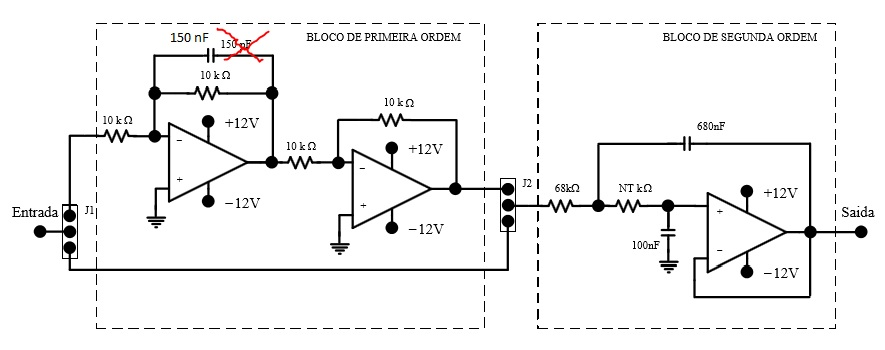
\includegraphics[scale=0.5]{./img/plantaProposta.jpg}
	\label{fig:plantaProposta_1}
	\legend{Fonte: Slide de apresentação do projeto}
\end{figure}

A \autoref{fig:esquematico_1} ilustra o esquemático da planta apresentada na \autoref{fig:plantaProposta_1} em conjunto com o sistema de controle formando um sistema em malha fechada.
A interface do sistema digital com o sistema analógico, no sentido do fluxo de sinal do sistema digital para o analógico, será feito com modulação de largura de pulso (PWM - Pulse Width Modulation). 
A interface no sentido do fluxo de sinal do sistema analógico para o sistema digital será feito por meio de conversores analógicos digitais.

\begin{figure}[htb!]
	\centering
	\caption{Esquemático do Sistema - Planta e Controlador.}
	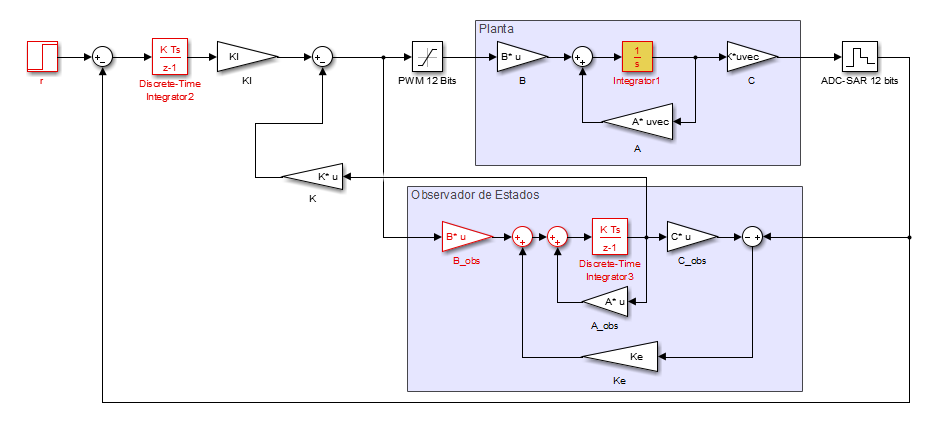
\includegraphics[scale=0.6]{./img/modeloSistemaDeControle_intro.PNG}
	\label{fig:esquematico_1}
	\legend{Software: MATLAB - Simulink}
\end{figure}

\pagebreak



\section{\textbf{Montagem da planta e sistema de controle.}}

\subsection{Montagem da planta em placa de circuito impresso.}
 
O layout da planta foi desenhado por meio do \textit{software} Altium. O amplificador operacional utilizado foi o LM224n. O layout abaixo segue o esquemático da \autoref{fig:plantaProposta_1} com um diodo zener 1N4734A de 5.6 V para proteção do ADC do microcontrolador contra tensão acima das suportadas pelo pino do microcontrolador (que segundo o \textit{datasheet} é 5.5 V para os microcontroladores da Cypress da linha PSOC 5LP).
Essa proteção é pertinente uma vez que os amplificadores operacionais irão operar com tensão simétrica de 12 V. 

\begin{figure}[htb!]
	\centering
	\caption{Layout da placa de circuito impresso.}
	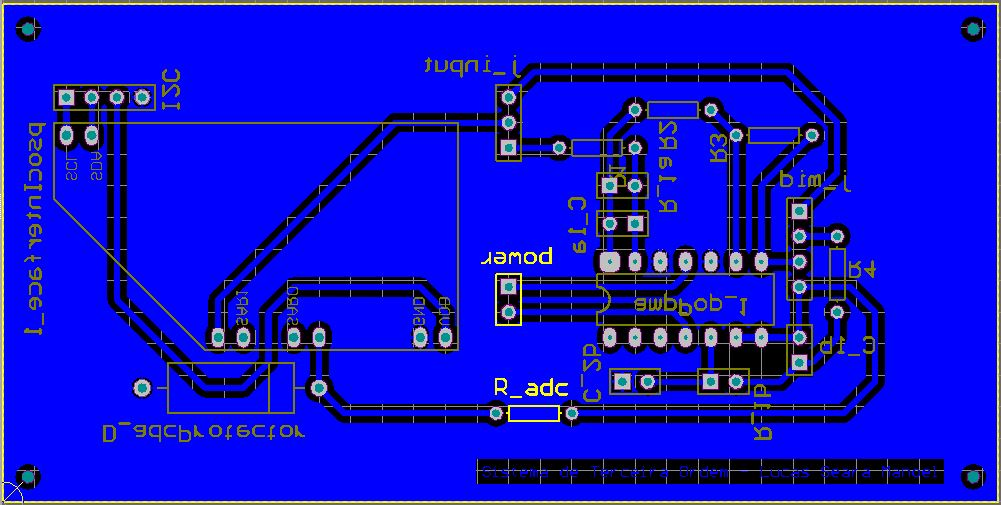
\includegraphics[scale=0.5]{./img/layout.JPG}
	\label{fig:layout}
	\legend{Software: Altium}
\end{figure}

A \autoref{fig:plantaMontagem_4.jpg} apresenta como ficou a placa de circuito impresso após corrosão. As dimensões da placa são 5x10 cm:

\begin{figure}[htb!]
	\centering
	\caption{Placa de circuito impresso após corrosão.}
	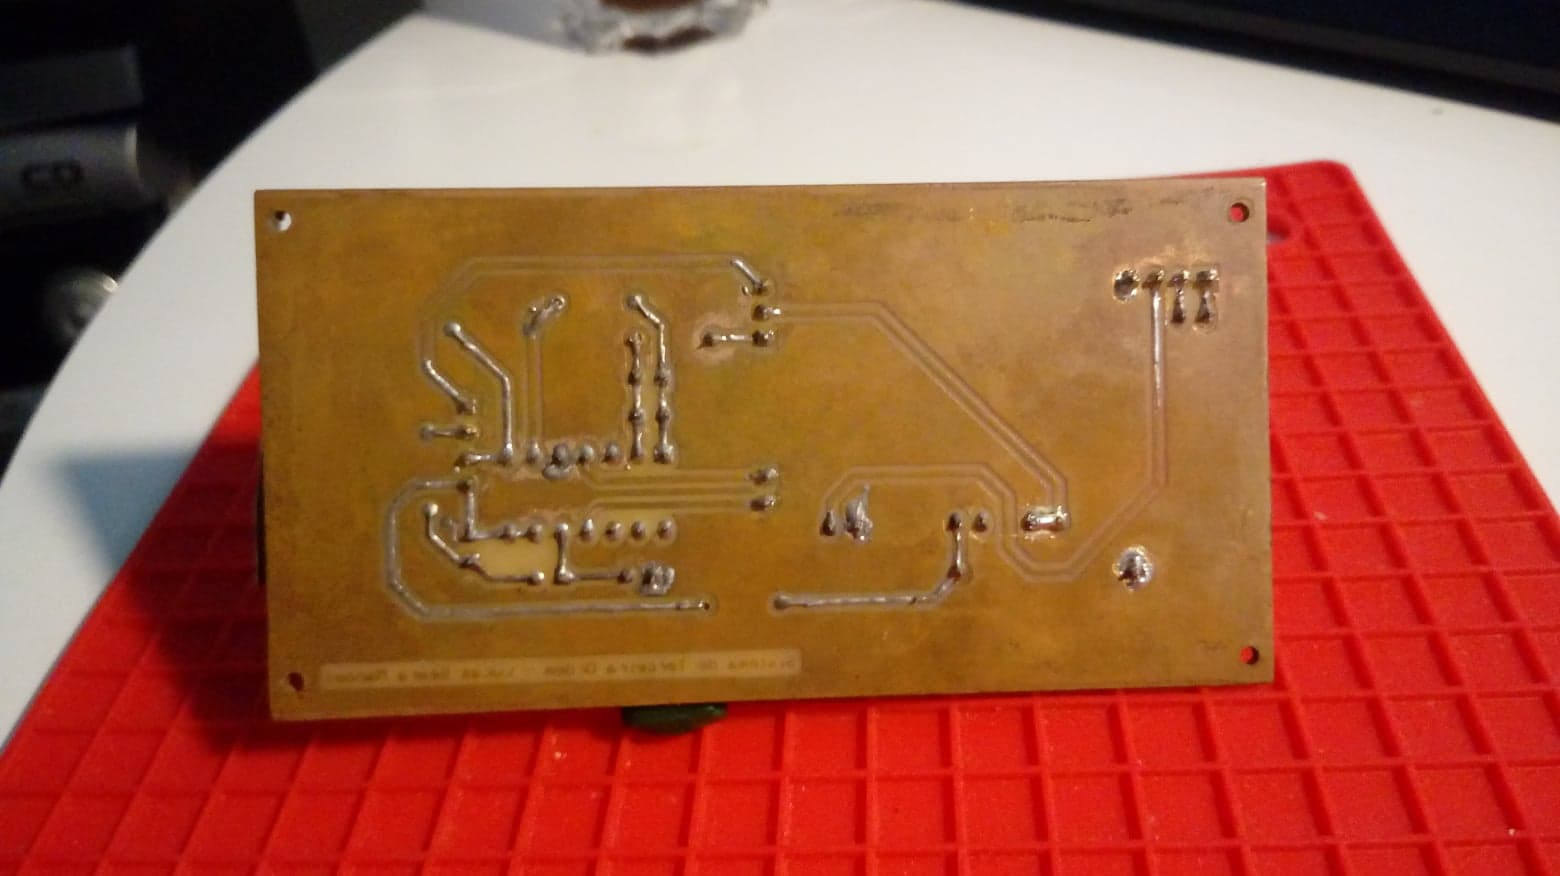
\includegraphics[scale=0.23]{./img/plantaMontagem_4.jpg}
	\label{fig:plantaMontagem_4.jpg}
\end{figure}

\pagebreak

O layout do da planta foi desenhado de forma que os elementos chaves que definem as constantes de tempo possam ser facilmente substituídos. 
Dessa forma é evitado que seja preciso reaquecer as trilhas de cobre da placa de fenolite em um processo de retrabalho de soldagem.
Essa abordagem facilitou a troca de um dos capacitores do sistema de primeira ordem que foi substituído durante o decorrer do projeto (essa troca está indicada com uma marcação X em vermelho na \autoref{fig:plantaProposta_1} - troca do capacitor de 150 pF para 150 nF). 

\begin{figure}[htb!]
	\centering
	\caption{Placa de circuito - Top Layer.}
	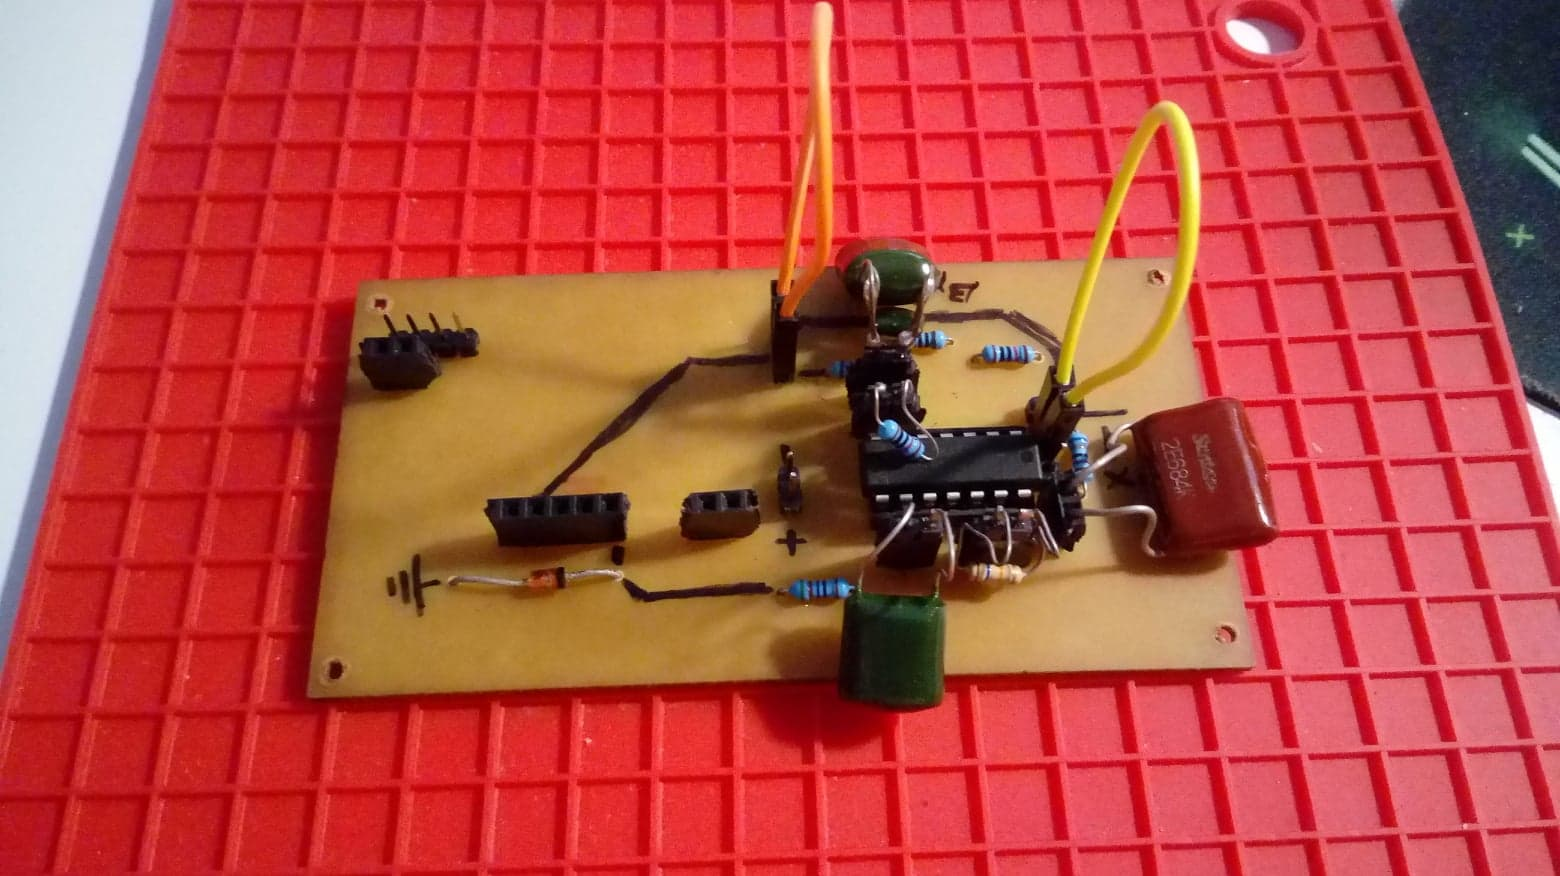
\includegraphics[scale=0.23]{./img/plantaMontagem_2.jpg}
	\label{fig:plantaMontagem_2}
\end{figure}

Para prevenir o mal contato entre os terminais dos componentes removíveis com a planta, foram soldados aos terminais dos componentes pinos que exercem um bom encaixe com os \textit{headers} da planta.
\begin{figure}[htb!]
	\centering
	\caption{Placa de circuito impresso - Componentes Removíveis.}
	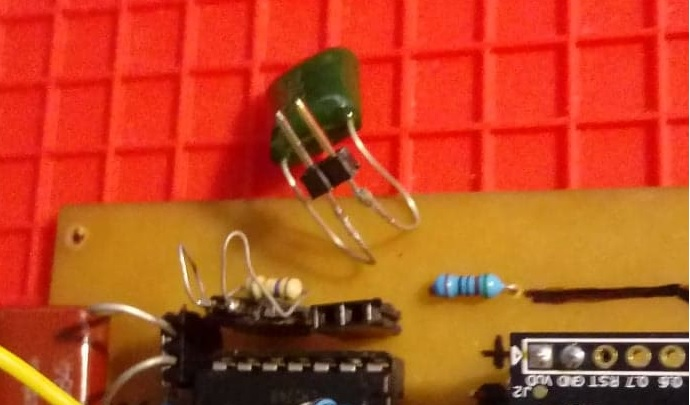
\includegraphics[scale=0.7]{./img/plantaMontagem_3.jpg}
	\label{fig:plantaMontagem_3}
\end{figure}

\pagebreak

\subsection{Implementação do sistema de controle com uso do dispositivo PSOC.}
\label{sec:implement_psoc}
O layout foi desenvolvido com base na placa de desenvolvimento CY8CKIT-059 da Cypress. 
Essa placa de desenvolvimento carrega um PSOC (\textit{Programable System On Chip}) da família CY8C58LP.
O dispositivo presente na placa é o CY8C5888LTI-LP097 que é um dispositivo que carrega um microcontrolador ARM Cortex-M3 em conjunto com periféricos que podem ter suas disposições programadas dentro do componente.

\begin{figure}[htb!]
	\centering
	\caption{Planta com Microcontrolador acoplado.}
	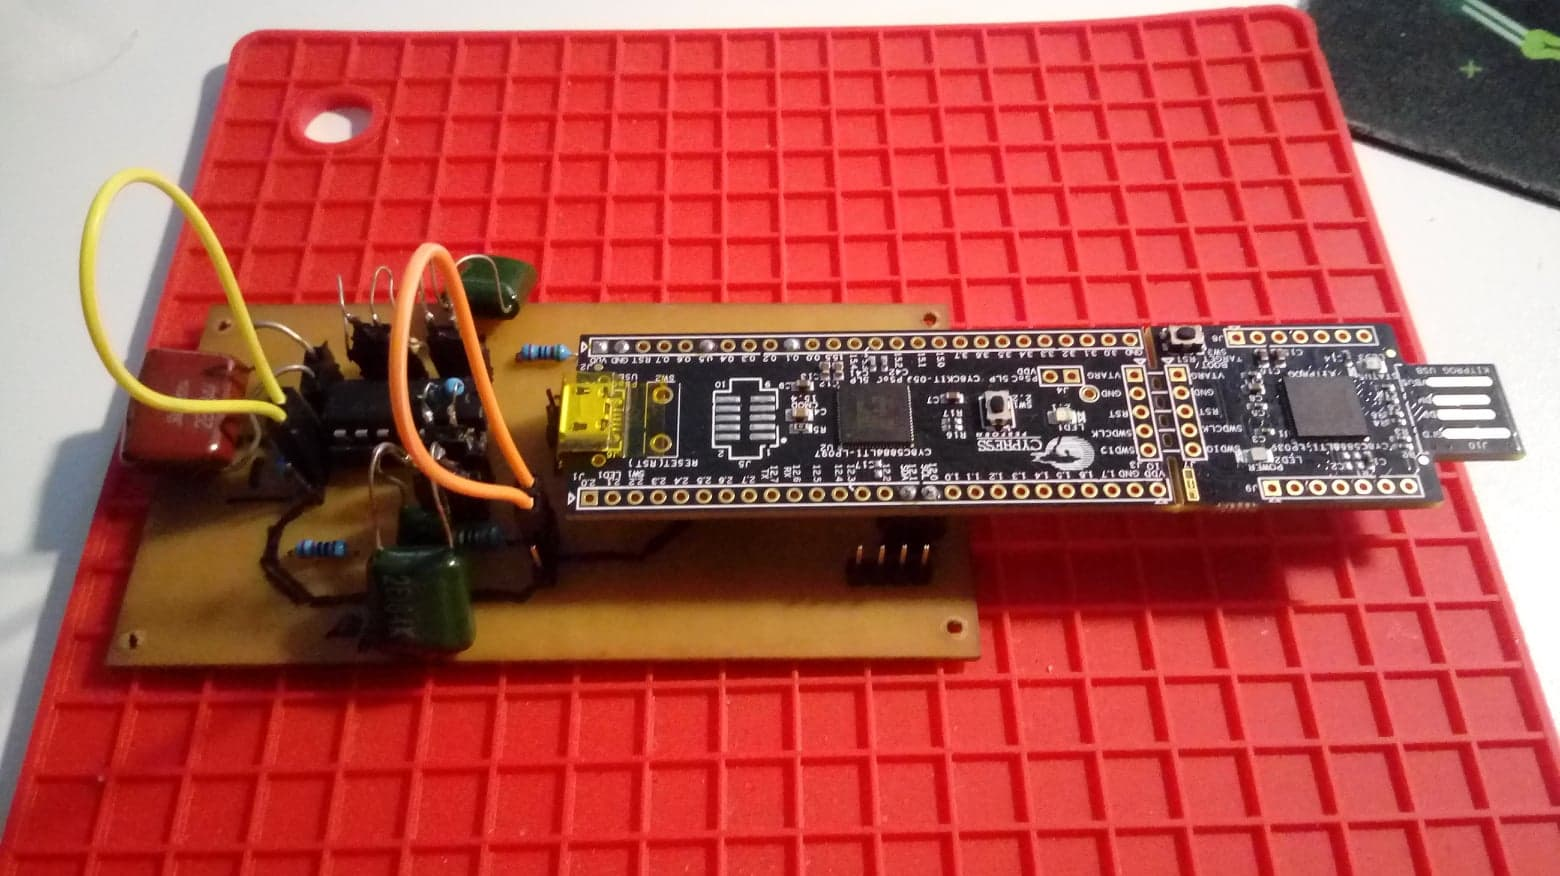
\includegraphics[scale=0.14]{./img/plantaMontagem_1.jpg}
	\label{fig:plantaMontagem_1}
\end{figure}

Esse componente possui vários periféricos disponíveis para uso, incluindo periféricos analógicos como amplificadores operacionais, comparadores, PGAs (amplificadores de ganho programável), TIAs (Amplificadores de Trans-impedância), Mixers e outros. Os principais periféricos utilizados nessa atividade foram o ADC SAR de 12 bits e um PWM também de 16 bits configurado exercer um período referente a 12 bits.
A \autoref{fig:PSOC5LP_features} retirada do \textit{datasheet} do componente mostra um mapa dos periféricos disponíveis:
\begin{figure}[htb!]
	\centering
	\caption{Mapa dos periféricos do PSOC da família CY8C58LP.}
	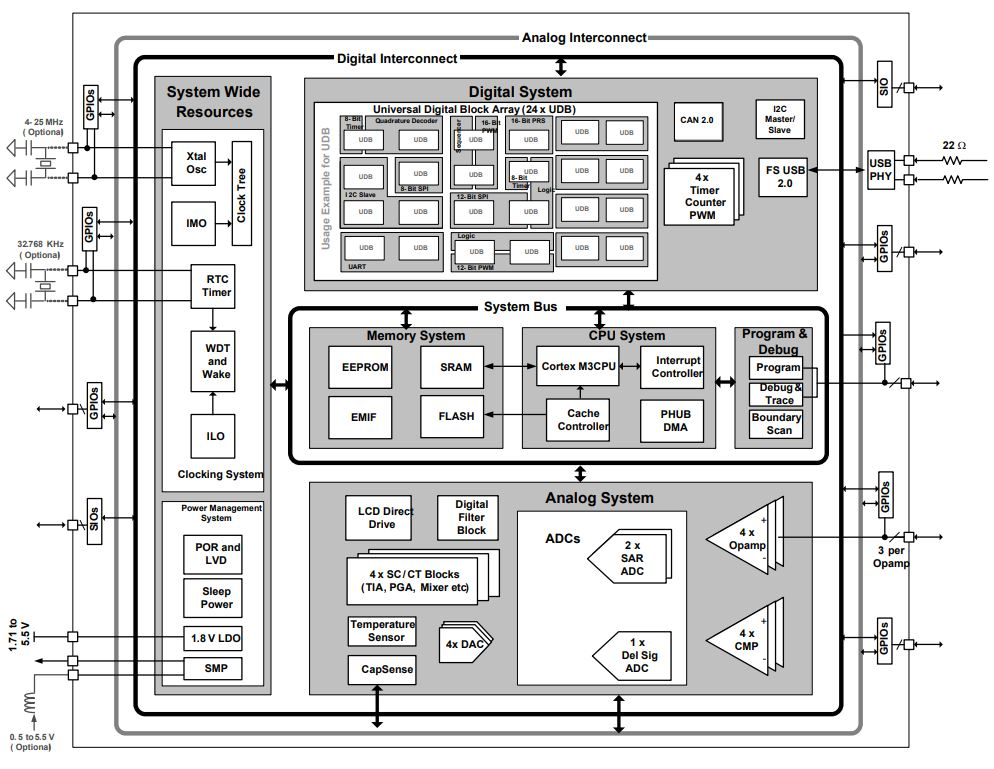
\includegraphics[scale=0.55]{./img/PSOC5LP_features.JPG}
	\label{fig:PSOC5LP_features}
\end{figure}

\pagebreak

A disposição dos periféricos é estabelecida via diagrama de blocos como o esquemático da \autoref{fig:PSOC_esquematico}.
A partir de um sinal de \textit{clock} de 66 MHz, sinais de \textit{clock} de menor frequência serão gerados para que o PWM seja sincronizado ao sinal de interrupção. Como o período do PWM está configurado para contar até 4096 ciclos, esse exercerá aproximadamente 16113 ações de controle por segundo.  
Periféricos como a interface UART também foram adicionados como também pode ser visto na \autoref{fig:PSOC_esquematico}:


\begin{figure}[htb!]
	\centering
	\caption{Esquemático dos periféricos implementados.}
	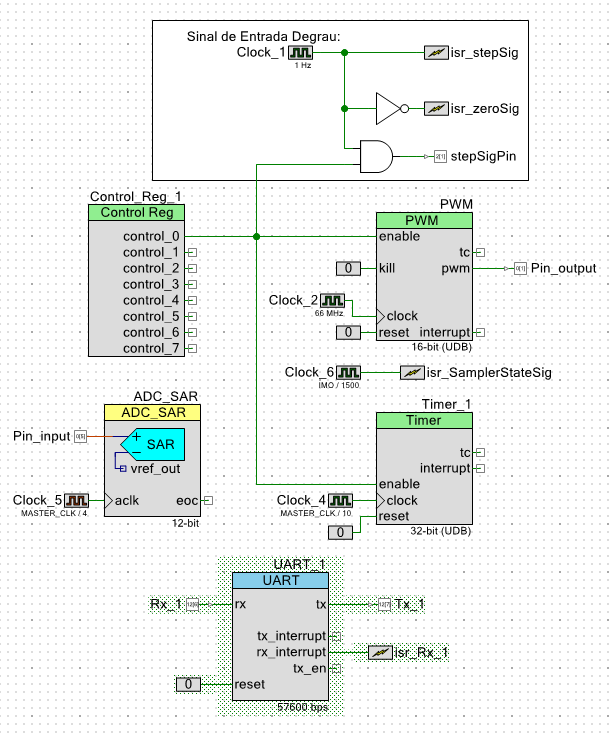
\includegraphics[scale=0.85]{./img/PSOC_esquematico.PNG}
	\label{fig:PSOC_esquematico}
	\legend{Software: PSoC Creator 4.2}
\end{figure}

O dispositivo PSOC irá implementar o hardware descrito na \autoref{fig:PSOC_esquematico}. O núcleo do processador ARM Cortex-M3 irá interagir com esse hardware por meio dos pinos de interrupção iniciados pela sigla isr. 
Logo a cada acionamento do pino de interrupção SamplerStateSig, uma função responsável por processar o sinal lido pelo ADC para atualizar o valor da saída PWM será chamada.
O sinal lido pelo ADC também é enviado via UART para que possa ser visualizado no computador.
O código completo do firmware está disponível no \autoref{app:firmwareCompleto}.

\pagebreak

O periférico conversor digital do tipo SAR foi configurado como é mostrado na \autoref{fig:ADCconfig}.
Operando com uma frequência de 16.5 MHz, o periférico está efetuando 916667 leituras por segundo - período de amostragem de 1.09 $\mu$s. 
Sendo a resolução de 12 bits, o erro de quantização é de $2^{-12} = 0.024\%$ que corresponde a uma relação sinal ruído de 72.25 dB.


\begin{figure}[htb!]
	\centering
	\caption{Medição do sobressinal do sistema de segunda ordem.}
	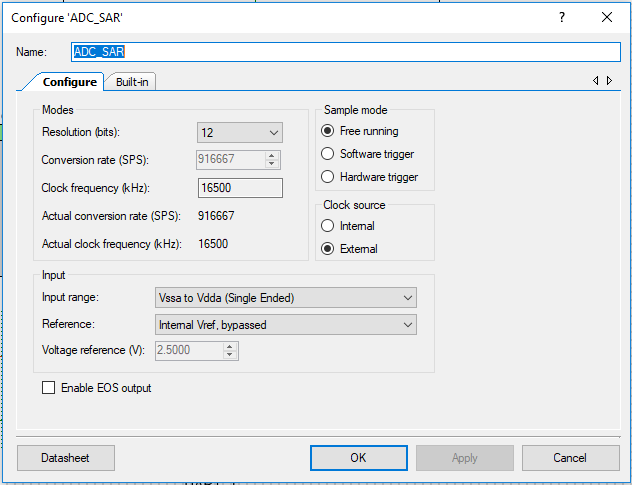
\includegraphics[scale=0.9]{./img/ADCconfig.PNG}
	\label{fig:ADCconfig}
	\legend{Software: PSoC Creator 4.2}
\end{figure}

\pagebreak

Periférico de PWM possui a mesma resolução do ADC utilizado.
Funcionando com um \textit{clock} de 66 MHz, período de um ciclo irá corresponder a 62.076 $\mu$s com um \textit{dutycycle} podendo representar 4096 valores diferentes.
A configuração do periférico de PWM é apresentada na \autoref{fig:PWMconfig}.

\begin{figure}[htb!]
	\centering
	\caption{Configuração do PWM.}
	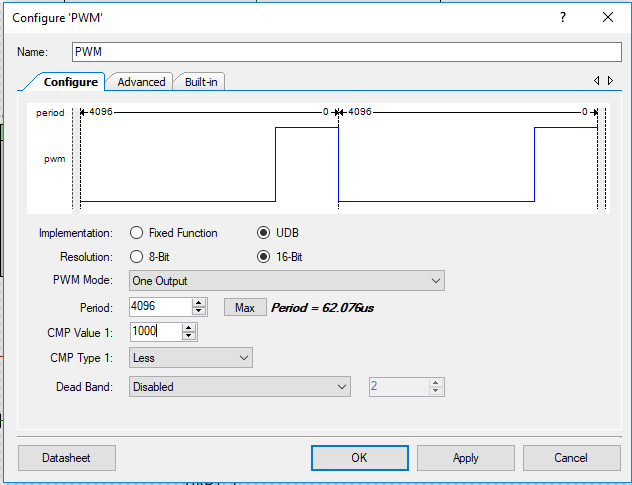
\includegraphics[scale=0.90]{./img/PWMconfig.PNG}
	\label{fig:PWMconfig}
	\legend{Software: PSoC Creator 4.2}
\end{figure}

\pagebreak

\section{\textbf{Análise da Planta.}}

\subsection{Modelagem da Planta.}

Para modelar a planta da \autoref{fig:planta_1} em uma representação de espaço de estados é preciso definir três variáveis de estado pois o sistema é de terceira ordem \cite{Ogata2014}. 
Logo é preciso extrair da planta três equações diferenciais de primeira, uma para cada estado, que englobam esses e suas respectivas derivadas. 
A equações diferencias extraídas devem se encaixar ao seguinte modelo do espaço de estados:

$$
\dot x = \textbf{A}x + \textbf{B}u
$$

$$
\left[
\begin{array}{ccc}
\dot x_1 \\
\dot x_2 \\
\dot x_3
\end{array}
\right]
 = 
A
\left[
\begin{array}{ccc}
x_1\\
x_2\\
x_3
\end{array}
\right]
+
B
u(t)
$$

Se for definido as tensões em cada capacitor como sendo uma variável de estado, a representação no espaço de estados assumirá a seguinte forma:

$$
\left[
\begin{array}{ccc}
\dot Vc_1 \\
\dot Vc_2 \\
\dot Vc_3
\end{array}
\right]
 = 
A
\left[
\begin{array}{ccc}
Vc_1\\
Vc_2\\
Vc_3
\end{array}
\right]
+
B
u(t)
$$

\begin{figure}[htb!]
	\centering
	\caption{Esquemático da Planta.}
	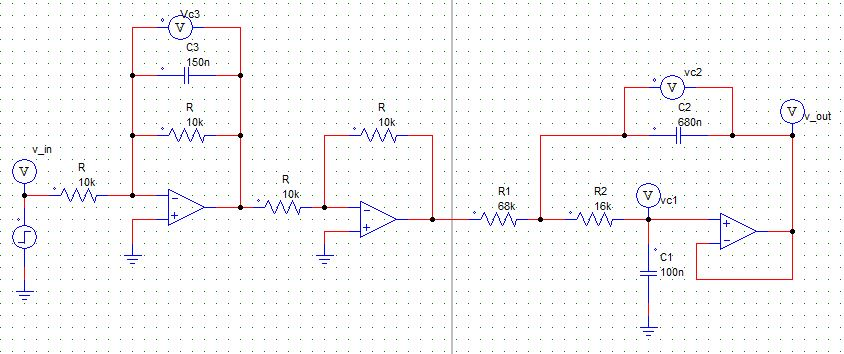
\includegraphics[scale=0.6]{./img/planta_1.JPG}
	\label{fig:planta_1}
	\legend{Software: PSIM}
\end{figure}

Com base na \autoref{fig:planta_1}, por meia das leis das correntes de Kirchhoff, as seguintes equações diferencias de primeira ordem foram extraídas da planta:
$$
	\dot V_{c1} = \frac{V_{c2}}{R_2C_2}
$$
$$
	\dot V_{c2} = -\frac{V_{c1}}{R_1C_2}-V_{c2}\frac{R_1+R_2}{R_1R_2C_2}+\frac{V_{c3}}{R_1C_2}
$$
$$
	\dot V_{c3} = -\frac{V_{c3}}{RC_3}+\frac{u(t)}{RC_3}
$$

$$
\left[
\begin{array}{ccc}
\dot Vc_1 \\
\dot Vc_2 \\
\dot Vc_3
\end{array}
\right]
 = 
\left[
\begin{array}{ccc}
0 & \frac{1}{R_2C_2} & 0 \\
-\frac{1}{R_1C_2} & -\frac{R_1+R_2}{R_1R_2C_2} &\frac{1}{R_1C_2} \\
0 & 0 & -\frac{1}{RC_3}
\end{array}
\right]
\left[
\begin{array}{ccc}
Vc_1\\
Vc_2\\
Vc_3
\end{array}
\right]
+
\left[
\begin{array}{ccc}
0 \\
0 \\
\frac{1}{RC_3}
\end{array}
\right]
u(t)
$$

\pagebreak

Além da relação da entrada com os estados do sistema, a representação do espaço de estados requer uma relação dos estados do sistema com a saída:
$$
y = \textbf{C}x + \textbf{D}u
$$
Como pode ser visto na \autoref{fig:planta_1}, a tensão no capacitor $C_1$ é espelhada para o sinal de saída. 
Logo os estado $Vc_1$ pode ser definido como saída e assim a relação pode ser definida da seguinte forma:
$$
y(t)=x_1=Vc_1
$$
$$
y(t)
=
\left[
\begin{array}{ccc}
1 & 0 & 0
\end{array}
\right]
\left[
\begin{array}{ccc}
x_1\\
x_2\\
x_3
\end{array}
\right]
=
\left[
\begin{array}{ccc}
1 & 0 & 0
\end{array}
\right]
\left[
\begin{array}{ccc}
Vc_1\\
Vc_2\\
Vc_3
\end{array}
\right]
$$

Logo as quatro matrizes da representação no espaço de estados da planta são definidas como:
$$
\textbf{A} = \left[
\begin{array}{ccc}
0 & \frac{1}{R_2C_2} & 0 \\
-\frac{1}{R_1C_2} & -\frac{R_1+R_2}{R_1R_2C_2} &\frac{1}{R_1C_2} \\
0 & 0 & -\frac{1}{RC_3}
\end{array}
\right]
= 
\left[
\begin{array}{ccc}
0 & 625 & 0 \\
-21.6263 & -113.5381 & 21.6263 \\
0 & 0 & -666.6667
\end{array}
\right]
$$

$$
\textbf{B} = 
\left[
\begin{array}{ccc}
0 \\
0 \\
\frac{1}{RC_3}
\end{array}
\right]
= 
\left[
\begin{array}{ccc}
0 \\
0 \\
666.6667
\end{array}
\right]
$$

$$
\textbf{C} = 
\left[
\begin{array}{ccc}
1 & 0 & 0
\end{array}
\right]
$$

$$
\textbf{D} = 0
$$

Ao analisar esse sistema por meio da função \textit{step()} do MATLAB é possível verificar o comportamento da resposta ao degrau desse sistema:

\begin{figure}[htb!]
	\centering
	\caption{Resposta ao degrau da representação no espaço de estados.}
	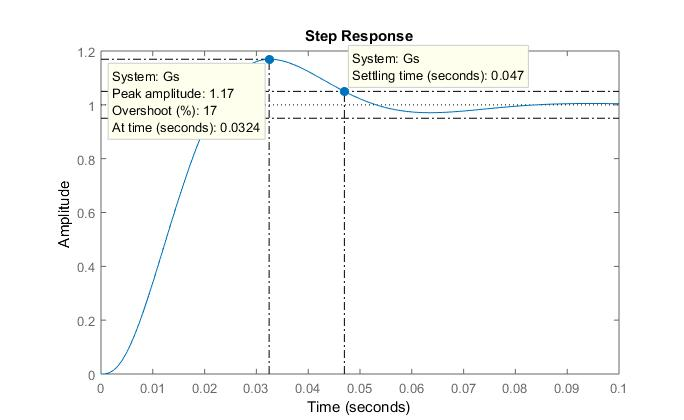
\includegraphics[scale=0.525]{./img/sistemaTerceiraOrdem_step.JPG}
	\label{fig:sistemaTerceiraOrdem_step}
	\legend{Software: MATLAB}
\end{figure}

\pagebreak

E a \autoref{fig:stepSimul}, sendo a simulação da planta por meio do \textit{software} PSIM, apresenta um resultado bem semelhante ao da simulação no MATLAB na \autoref{fig:sistemaTerceiraOrdem_step}.

\begin{figure}[htb!]
	\centering
	\caption{Resposta ao degrau da planta da \autoref{fig:planta_1}.}
	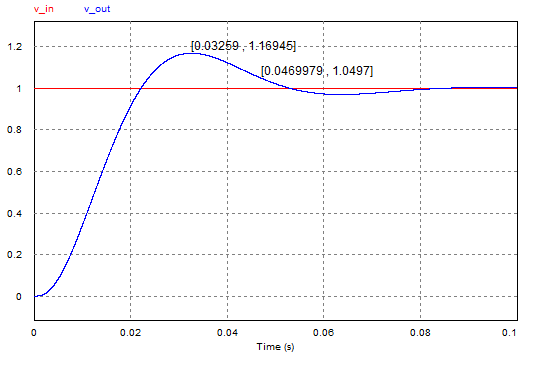
\includegraphics[scale=0.75]{./img/stepSimul.PNG}
	\label{fig:stepSimul}
	\legend{Software: PSIM}
\end{figure}

Com o PSIM é possível também fazer uma medição dos estados da planta, as tensões em cada capacitor:

\begin{figure}[htb!]
	\centering
	\caption{Resposta ao degrau da planta da \autoref{fig:planta_1}.}
	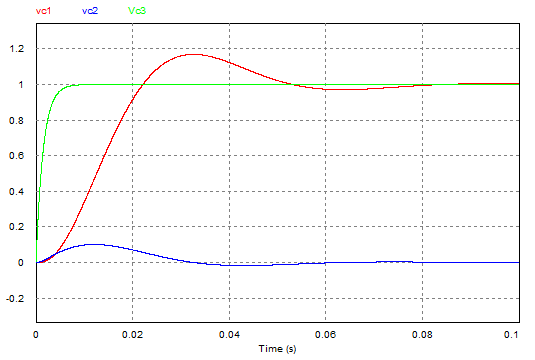
\includegraphics[scale=0.75]{./img/stepSimul_estados.PNG}
	\label{fig:stepSimul_estados}
	\legend{Software: PSIM}
\end{figure}

\pagebreak

Para comparar os estados da planta simulados no PSIM com os estados do modelo do MATLAB, o simulink permite fazer a leitura dos três estados na saída do integrado do modelo no espaço de estados (\autoref{fig:simulink_esquematicoPlantaSS}). É possível ver a semelhança entre a \autoref{fig:stepSimul_estados} e a \autoref{fig:simulink_estados}.

\begin{figure}[htb!]
	\centering
	\caption{Modelo no espaço de estados da \autoref{fig:planta_1}.}
	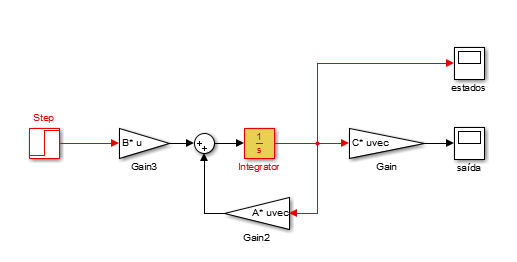
\includegraphics[scale=0.75]{./img/simulink_esquematicoPlantaSS.PNG}
	\label{fig:simulink_esquematicoPlantaSS}
	\legend{Software: MATLAB}
\end{figure}

\begin{figure}[htb!]
	\centering
	\caption{Resposta ao degrau da planta da \autoref{fig:planta_1}.}
	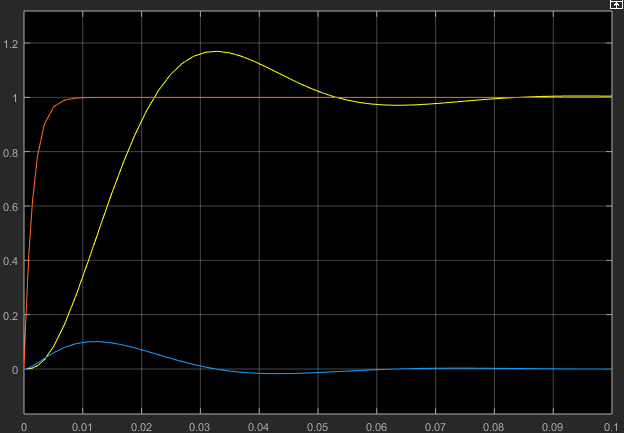
\includegraphics[scale=0.75]{./img/simulink_estados.PNG}
	\label{fig:simulink_estados}
	\legend{Software: MATLAB}
\end{figure}

\pagebreak

\subsection{Teste de Controlabilidade.}

O sistema é dito completamente controlável se o posto da matriz de controlabilidade de dimensão $n\timesn$ for igual a $n$\cite{Ogata2014}:
$$
M_{controlabilidade} = 
\left[
\begin{array}{c;{2pt/2pt}c;{2pt/2pt}c}
\textbf{B} & \textbf{AB} & \textbf{A}^{2}\textbf{B}
\end{array}
\right]
$$

$$
\textbf{AB} = 
\left[
\begin{array}{ccc}
0 \\
1.4428*10^{4}\\
-4.4444*10^{5}
\end{array}
\right]
$$

$$
\textbf{A}^{2}\textbf{B} = 
\left[
\begin{array}{ccc}
9.0109*10^{6}\\
-1.1125*10^{7}\\
2.9629*10^{8}
\end{array}
\right]
$$

$$
M_{controlabilidade} = 
\left[
\begin{array}{c;{2pt/2pt}c;{2pt/2pt}c}
\textbf{B} & \textbf{AB} & \textbf{A}^{2}\textbf{B}
\end{array}
\right]
=
\left[
\begin{array}{c;{2pt/2pt}c;{2pt/2pt}c}
0 & 0 & 9.0109*10^{6}\\
0 & 1.4428*10^{4} & -1.1125*10^{7}\\
666.6667 & -4.4444*10^{5} & 2.9629*10^{8}
\end{array}
\right]
$$
Logo como a matriz de controlabilidade possui $n=3$ e posto $3$, o sistema é completamente controlável.
Como o sistema possui apenas uma saída, o posto da matriz de controlabilidade de saída precisa ter posto igual a 1. E isso pode ser conferido da seguinte forma:
$$
M_{saída} = 
\left[
\begin{array}{c;{2pt/2pt}c;{2pt/2pt}c}
\textbf{CB} & \textbf{CAB} & \textbf{CA}^{2}\textbf{B}
\end{array}
\right]
$$

$$
\textbf{CB} = 
\left[
\begin{array}{ccc}
0 
\end{array}
\right]
$$

$$
\textbf{CAB} = 
\left[
\begin{array}{ccc}
0 
\end{array}
\right]
$$

$$
\textbf{CA}^{2}\textbf{B} = 
\left[
\begin{array}{ccc}
9.0109*10^{6}
\end{array}
\right]
$$

$$
M_{saída} = 
\left[
\begin{array}{c;{2pt/2pt}c;{2pt/2pt}c}
\textbf{CB} & \textbf{CAB} & \textbf{CA}^{2}\textbf{B}
\end{array}
\right]
=
\left[
\begin{array}{c;{2pt/2pt}c;{2pt/2pt}c}
0 & 0 & 9.0109*10^{6}
\end{array}
\right]
$$

\pagebreak

\subsection{Teste de Observabilidade.}

O sistema é dito completamente observável se o posto da matriz de observabilidade de dimensão $n\timesn$ for igual a $n$ \cite{Ogata2014}:
$$
M_{observabilidade} = 
\left[
\begin{array}{c;{2pt/2pt}c;{2pt/2pt}c}
\textbf{C}^* & \textbf{A}^*\textbf{C}^* & (\textbf{A}^*)^{2}\textbf{C}^*
\end{array}
\right]
$$

$$
\textbf{C}^* = 
\left[
\begin{array}{ccc}
1 \\
0\\
0
\end{array}
\right]
$$

$$
\textbf{A}^*\textbf{C}^* = 
\left[
\begin{array}{ccc}
0 \\
625\\
0
\end{array}
\right]
$$

$$
(\textbf{A}^*)^{2}\textbf{C}^* = 
\left[
\begin{array}{ccc}
-1.3516*10^{4}\\
-7.0961*10^{4}\\
1.3516*10^{4}
\end{array}
\right]
$$

$$
M_{observabilidade} = 
\left[
\begin{array}{c;{2pt/2pt}c;{2pt/2pt}c}
\textbf{C}^* & \textbf{A}^*\textbf{C}^* & (\textbf{A}^*)^{2}\textbf{C}^*
\end{array}
\right]
=
\left[
\begin{array}{c;{2pt/2pt}c;{2pt/2pt}c}
1 & 0 & -1.3516*10^{4}\\
0 & 625 & -7.0961*10^{4}\\
0 & 0 & 1.3516*10^{4}
\end{array}
\right]
$$

Logo como a matriz de observabilidade possui $n=3$ e posto $3$, dessa forma o sistema é completamente observável. Essa característica indica que será possível implementar um observador de estados \cite{Ogata2014}.

\pagebreak

\subsection{Erro de Regime Permanente.}

Por meio do teorema do valor final é possível verificar o erro de regime permanente por meio da equação de erro da planta no domínio da frequência complexa \cite{lathi2014}:

$$
\lim_{s\to0} sE(s) = e(\infty)=\lim_{s\to0} sR(s)(1 - \textbf{C}(s\textbf{I}-\textbf{A})^{-1}\textbf{B})
$$
Para verificar o erro de regime permanente para a entrada degrau:$R(s)=\frac{1}{s}$
$$
e(\infty)=\lim_{s\to0} (1 - \textbf{C}(s\textbf{I}-\textbf{A})^{-1}\textbf{B}) = 1 - \textbf{C}\textbf{A}^{-1}\textbf{B}
$$

$$
1 - \textbf{C}\textbf{A}^{-1}\textbf{B} = 
1 -
\left[
\begin{array}{ccc}
1 & 0 & 0
\end{array}
\right]
*
\left[
\begin{array}{ccc}
0 & -21.6263 & 0\\
625 & -113.5381 & 0\\
0 & 21.6263 & -666.6667
\end{array}
\right]
*
\left[
\begin{array}{ccc}
0 \\
0 \\
666.6667
\end{array}
\right]
= 
2
$$

$$
e(\infty)=1 - \textbf{C}\textbf{A}^{-1}\textbf{B} = 2
$$

Logo é verificado que a planta possui erro de regime permanente igual a dois. Assim sendo uma planta do tipo 0 \cite{Ogata2014}.
\pagebreak

\section{\textbf{Projeto de Controlador no Espaço de Estados por alocação de polos}}

A ideia básica de um controlador projetado no espaço de estados por realocação de polos consiste por meia da realimentação de estados a alteração da constante de tempo do sistema. É possível visualizar essa ideia entre o paralelo da solução da equação diferencial de primeira ordem na forma escalar e matricial:
$$
\dot x = ax + bu
$$
$$
\mathscr{L}\{\dot x = bx + au\}=sX(s)-x(0)=aX(s)+bU(s)
$$
$$
u = -kx
$$
$$
\dot x = ax - bkx = x(a - bk)
$$
$$
\mathscr{L}\{\dot x = x(a - bk)\}=sX(s)-x(0)=(a - bk)X(s)
$$
$$
X(s)=\frac{x(0)}{(s-a + bk))}
$$
$$
\mathscr{L}^{-1}\{X(s)\}=x(t)=e^{(a-bk)t}x(0)
$$

$$
\dot x = \textbf{A}x + \textbf{B}u
$$
$$
u = -\textbf{K}x
$$
$$
\dot x = \textbf{A}x - \textbf{B}\textbf{K}x = (\textbf{A} - \textbf{B}\textbf{K})x
$$
$$
x(t)=e^{(\textbf{A}-\textbf{BK})t}x(0)
$$

Logo pela realimentação de estados, como apresentado no esquemático da \autoref{fig:regulador_1}, é possível realocar os polos do sistema.

\begin{figure}[htb!]
	\centering
	\caption{Esquemático do Sistema Regulador em malha fechada.}
	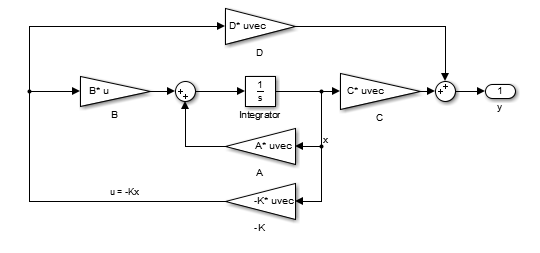
\includegraphics[scale=1]{./img/regulador_1.PNG}
	\label{fig:regulador_1}
	\legend{Software: Simulink}
\end{figure}

\pagebreak

Para que o sistema possa ter sua referência alterada e deixe de ser um sistema regulador para se tornar um servossistema, o valor de referência $r$ precisa ser modelado junto ao sistema.

\begin{figure}[htb!]
	\centering
	\caption{Esquemático do servossistema no espaço de estados.}
	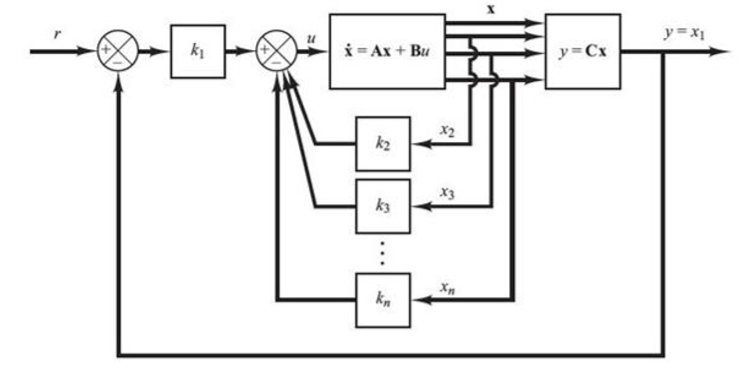
\includegraphics[scale=0.8]{./img/servossitema.PNG}
	\label{fig:servossitema}
	\legend{Livro: \cite{Ogata2014}}
\end{figure}

$$
u
=
-
\left[
\begin{array}{ccc}
0 & k_2 & k_3
\end{array}
\right]
\left[
\begin{array}{ccc}
x_1\\
x_2\\
x_3
\end{array}
\right]
+
k_1(r-x_1)
=
-\textbf{Kx}+k_1r
$$
$$
\dot x = \textbf{A}x - \textbf{B}u = x(\textbf{A} - \textbf{BK}) + \textbf{B}k_1r
$$

$$
\dot x(t) - \dot x(\infty) = (x(t)-x(\infty))(\textbf{A} - \textbf{BK}) + \textbf{B}k_1(r(t)-r(\infty))
$$
$$
r(t)=r(\infty)
$$
$$
\dot x(t) - \dot x(\infty) = (x(t)-x(\infty))(\textbf{A} - \textbf{BK})
$$
$$
\dot e(t) = (\textbf{A} - \textbf{BK})e(t)
$$
Logo se baseando pelo erro, o projeto do servossistema é convertido para um projeto por alocação de polos de um regulador assintoticamente estável \cite{Ogata2014}.

\pagebreak

Como o planta apresenta um erro ao degrau, é necessário a adição de um integrador para que a planta se torne do tipo 1. Isso é possível expandindo a matriz:
$$
\left[
\begin{array}{c}
\dot \textbf{x(t)} \\
\dot \xi(t)
\end{array}
\right]
 = 
\left[
\begin{array}{cc}
\textbf{A} & \textbf{0}\\
\textbf{-C} & 0
\end{array}
\right]
\left[
\begin{array}{c}
\textbf{x(t)}\\
\xi(t)
\end{array}
\right]
+
\left[
\begin{array}{c}
\textbf{B}\\
0
\end{array}
\right]
u(t)
+
\left[
\begin{array}{c}
\textbf{0}\\
1
\end{array}
\right]
r(t)
$$

$$
\hat{A} = 
\left[
\begin{array}{cc}
\textbf{A} & \textbf{0}\\
\textbf{-C} & 0
\end{array}
\right]
$$

$$
\hat{B} = 
\left[
\begin{array}{cc}
\textbf{A} & \textbf{0}\\
\textbf{-C} & 0
\end{array}
\right]
$$

$$
\left[
\begin{array}{c}
\dot x(t) - \dot x(\infty) \\
\dot \xi(t) - \dot \xi(\infty)
\end{array}
\right]
 = 
\hat{A}
\left[
\begin{array}{c}
x(t) - x(\infty)\\
\xi(t) - \xi(\infty)
\end{array}
\right]
+
\hat{B}
(u(t)-u(\infty))
+
\left[
\begin{array}{c}
\textbf{0}\\
1
\end{array}
\right]
(r(t)-r(\infty))
$$

$$
r(t)=r(\infty)
$$

$$
\left[
\begin{array}{c}
\dot x(t) - \dot x(\infty) \\
\dot \xi(t) - \dot \xi(\infty)
\end{array}
\right]
 = 
\hat{A}
\left[
\begin{array}{c}
x(t) - x(\infty)\\
\xi(t) - \xi(\infty)
\end{array}
\right]
+
\hat{B}
(u(t)-u(\infty))
$$

$$
\left[
\begin{array}{c}
\dot x_e(t) \\
\dot \xi_e(t)
\end{array}
\right]
 = 
\hat{A}
\left[
\begin{array}{c}
x_e(t)\\
\xi_e(t)
\end{array}
\right]
+
\hat{B}
u_e(t)
$$

$$
e(t)=
\left[
\begin{array}{c}
x_e(t)\\
\xi_e(t)
\end{array}
\right]
$$

$$
\dot e(t)
 = 
\hat{A}
e(t)
+
\hat{B}
u_e(t)
$$

$$
u_e(t) = -\hat{K}e(t)
$$
Assim é possível executar o projeto por alocação de polos:
$$
\dot e(t)=(\hat{A}-\hat{B}\hat{K})e(t)
$$
$$
\hat{K}
=
\left[
\begin{array}{c;{2pt/2pt}c}
\textbf{K} & -k_i
\end{array}
\right]
=
\left[
\begin{array}{ccc;{2pt/2pt}c}
K_1 & K_2 & K_3 & -k_i
\end{array}
\right]
$$

$$
\hat{K}
=
\left[
\begin{array}{cccc}
0 & 0 & 0 & 1
\end{array}
\right]
\left[
\begin{array}{c;{2pt/2pt}c;{2pt/2pt}c;{2pt/2pt}c}
\textbf{B} & \textbf{AB}  & \textbf{A}^2\textbf{B}  & \textbf{A}^3\textbf{B} 
\end{array}
\right]^{-1}
\phi(\textbf{A}) 
$$
Onde $\phi(\textbf{A})$ é definido por meio dos polos de determinada localização onde no qual são desejados que sejam dominantes no sistema. 

\pagebreak

Como é desejador realocar os polos para uma posição desejada, podemos definir essa posição por meio de valores desejados de $\zeta$ e $t_s$. Os polos desejados foram calculados da seguinte forma \cite{Ogata2014}:
$$
\zeta = 0.75
$$
$$
t_s = 20 ms
$$
$$
\omega_n = \frac{3}{\zeta t_s}
$$
$$
\mu_1_{real} = \mu_2_{real} = \zeta \omega_n = 150
$$
$$
\mu_1_{imag} = \omega_n = 214.2857
$$
$$
\mu_2_{imag} = -\omega_n -214.2857
$$
$$
j=
\left[
\begin{array}{cccc}
\mu_1 &  \mu_2 & -1000 & -1000
\end{array}
\right]
=
\left[
\begin{array}{cccc}
150+j214.2857 &  150-j214.2857 & -1000 & -1000
\end{array}
\right]
$$
Como o MATLAB fornece uma função para calcular os ganhos K por meio da fórmula de Arkermann. Logo para os polos desejados:
$$
j=
\left[
\begin{array}{cccc}
\mu_1 &  \mu_2 & -1000 & -1000
\end{array}
\right]
$$
$$
\hat{K}
=
\left[
\begin{array}{ccc;{2pt/2pt}c}
43.8851 & 97.1551 & 2.2797 &  6.9360*10^{3}
\end{array}
\right]
=
\left[
\begin{array}{c;{2pt/2pt}c}
\textbf{K} & -k_i
\end{array}
\right]
=
\left[
\begin{array}{ccc;{2pt/2pt}c}
K_1 & K_2 & K_3 & -k_i
\end{array}
\right]
$$

$$
\dot \textbf{x}
 = 
\left[
\begin{array}{cc}
\textbf{A-BK} & \textbf{B}k_i\\
\textbf{-C} & 0
\end{array}
\right]
\textbf{x}
+
\left[
\begin{array}{cc}
\textbf{0}\\
1
\end{array}
\right]
u(t)
$$

$$
y
 = 
\left[
\begin{array}{cc}
\textbf{C} & 0
\end{array}
\right]
\textbf{x}
$$

\begin{figure}[htb!]
	\centering
	\caption{Resposta ao degrau do sistema compensado.}
	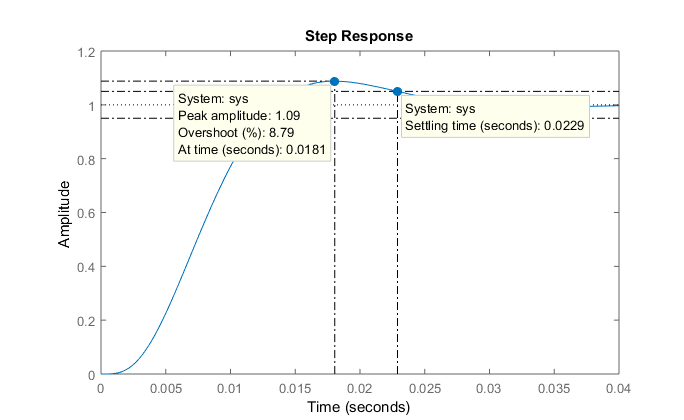
\includegraphics[scale=0.8]{./img/stepCtrl_1.png}
	\label{fig:stepCtrl_1}
	\legend{Software: MATLAB}
\end{figure}

\pagebreak

Como no caso dessa planta não é possível fazer a leitura de todos os estados do sistema, é necessário a implementação de um observador de estados. O projeto dessa implementação também pode ser feito por alocação de polos:
$$
\dot{\tilde{x}}=
\textbf{A}\tilde{x} + \textbf{B}u - (y - \textbf{C}\tilde{x})\textbf{K}_e=
(\textbf{A} - \textbf{C}\textbf{K}_e)\tilde{x} + \textbf{B}u + \textbf{K}_ey
$$
$$
\dot{x} - \dot{\tilde{x}}=
\textbf{A}\tilde{x} - \textbf{A}x - (\textbf{C}x - \textbf{C}\tilde{x})\textbf{K}_e=
(\textbf{A} - \textbf{C}\textbf{K}_e)(\tilde{x} - x)
$$
$$
e = x - \tilde{x}
$$
$$
\dot{e} = (\textbf{A} - \textbf{C}\textbf{K}_e)e
$$
A ideia é que o observador de estados tenha um sinal de erro que o faça seguir os estados da planta. Logo esse sinal de erro deve corrigir os estados observador mais rápido que a dinâmica da planta. Assim seus polos devem ser realocados afim de se tornarem mais rápidos que a planta. 

\begin{figure}[htb!]
	\centering
	\caption{Resposta ao degrau do sistema compensado.}
	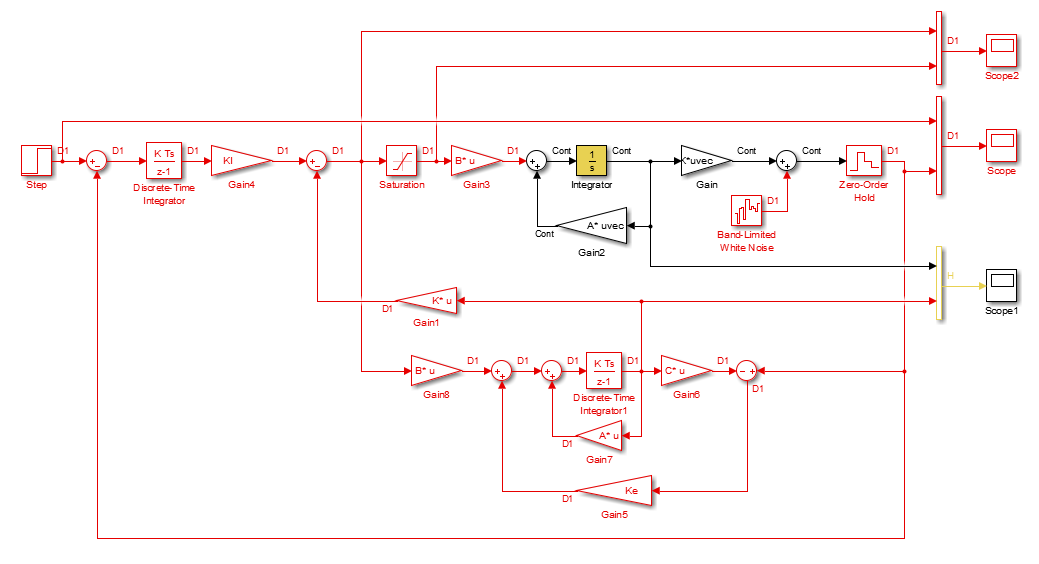
\includegraphics[scale=0.6]{./img/simulink_esquematicoCtrlObs.PNG}
	\label{fig:simulink_esquematicoCtrlObs}
	\legend{Software: Simulink}
\end{figure}

Como o ganho de erro do observador é uma coluna, a matriz A, C e o vetor de polos desejados devem ser utilizadas na forma transposta para que a fórmula de Ackermann retorne um vetor coluna de ganhos. A valor dos polos do observador foram considerados como duas vezes os polos desejados anteriormente calculados.

$$
j_{obs}= 2*j'
$$

$$
\textbf{K}_e
=
\left[
\begin{array}{c}
 319,7676\\
 482.0572\\
 4740.4562
\end{array}
\right]
$$

\pagebreak

\subsection{Análise em simulação do controlador.}

Observando a simulação da planta com controlador baseado no observador de estados, é possível ver que a amplitude do sobressinal passou um pouco o valor de requisito de projeto.

\begin{figure}[htb!]
	\centering
	\caption{Resposta ao degrau do sistema compensado.}
	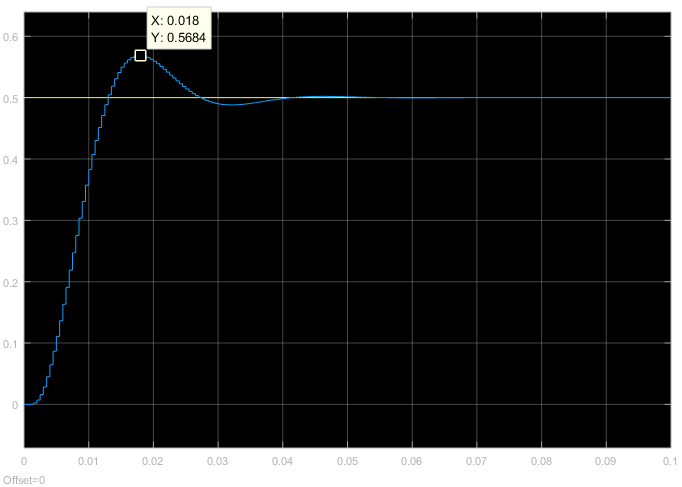
\includegraphics[scale=0.55]{./img/stepCtrlObs_1.png}
	\label{fig:stepCtrlObs_1}
	\legend{Software: Simulink}
\end{figure}

Com o ajuste do valor de $\zeta$ foi possível baixar um pouco o valor do sobressinal para um valor menor que o requisito de projeto:
$$
\zeta = 0.85
$$
$$
t_s = 20 ms
$$
$$
j=
\left[
\begin{array}{cccc}
150+j176.5 &  150-j176.5 & -1000 & -1000
\end{array}
\right]
$$

\begin{figure}[htb!]
	\centering
	\caption{Resposta ao degrau do sistema compensado após ajuste do $\zeta$.}
	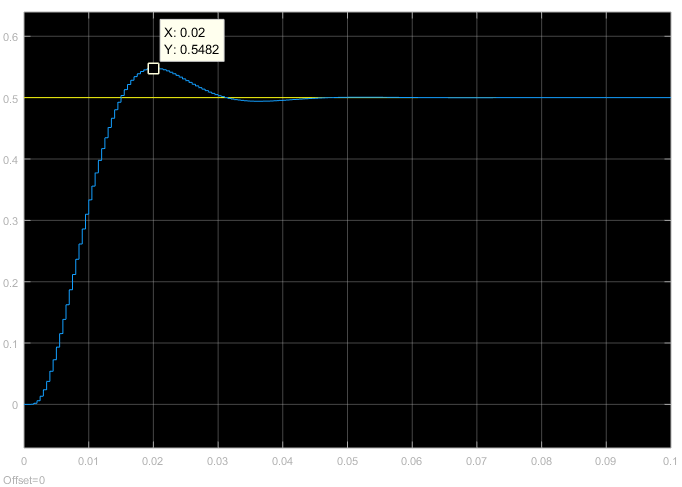
\includegraphics[scale=0.55]{./img/stepCtrlObs_ajustado_1.png}
	\label{fig:stepCtrlObs_ajustado_1}
	\legend{Software: Simulink}
\end{figure}

\pagebreak

Como pode ser visto na \autoref{fig:stepCtrlObs_wng_1}, um teste interessante para ser feito no Simulink é do desempenho da controlador com o acréscimo de ruído branco na entrada do ADC.

\begin{figure}[htb!]
	\centering
	\caption{Resposta ao degrau do sistema compensado com adição de ruído WNG}
	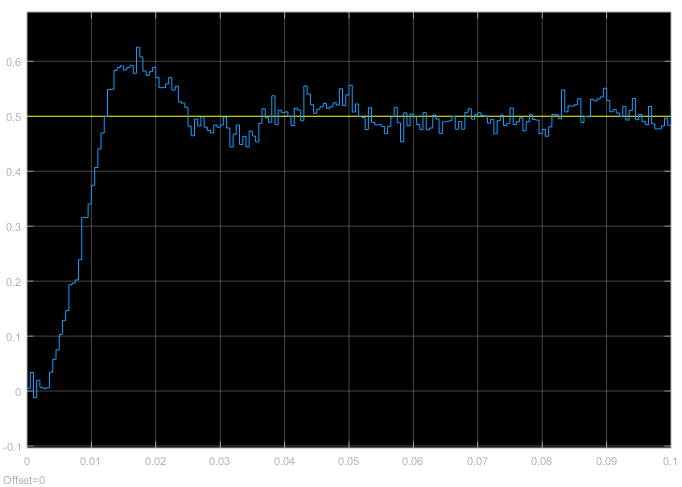
\includegraphics[scale=0.55]{./img/stepCtrlObs_wng_1.png}
	\label{fig:stepCtrlObs_wng_1}
	\legend{Software: Simulink}
\end{figure}

É possível notar que o requisito de projeto deixa de ser atendido com o acréscimo de ruído branco pois a ação de controle começa a atingir amplitudes maiores que a capacidade de representação do PWM. 
Na \autoref{fig:stepCtrlObs_wng_ctrlAction} é possível ver em amarelo o sinal da ação de controle antes da saturação e em azul depois de ser saturado. Isso fez com que o controlador na atingisse os requisitos de projeto.

\begin{figure}[htb!]
	\centering
	\caption{Ação de controle apresentado saturação.}
	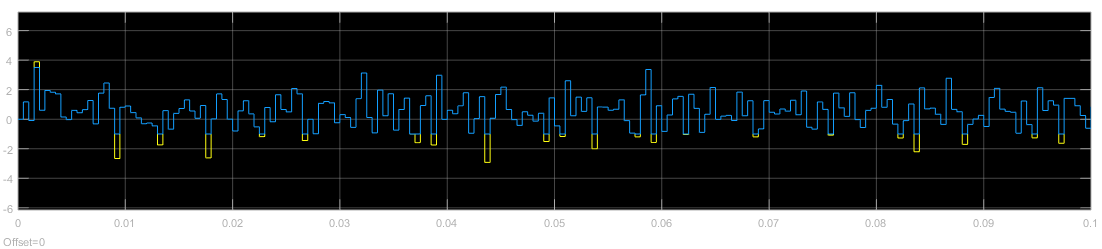
\includegraphics[scale=0.6]{./img/stepCtrlObs_wng_ctrlAction.png}
	\label{fig:stepCtrlObs_wng_ctrlAction}
	\legend{Software: Simulink}
\end{figure}

\pagebreak

Pelo fato controlador, por ser de quarta ordem, necessitar de quatro polos, mas é desejado apenas um par de polos dominantes, os demais são definidos com valores altos para que não interfiram. Porém se os valores desses polos forem muito grandes a banda passante do sistema se torna proporcionalmente grande fazendo com que o sistema seja mais vulnerável ao ruído. Abaixando o valor desses polos de $-1000$ para $-250$ é possível diminuir a sensibilidade do sistema ao ruído branco. Dessa forma foi resolvido o problema da alta amplitude da ação de controle que ocasionava a saturação do mesmo. Também foi possível baixar o valor de $\zeta$. Isso pode ser verificado na \autoref{fig:stepCtrlObs_ajustado_2} e \autoref{fig:stepCtrlObs_wng_ajustado_ctrlAction}:
$$
\zeta = 0.60
$$
$$
t_s = 20 ms
$$
$$
j=
\left[
\begin{array}{cccc}
150+j176.5 &  150-j176.5 & -250 & -250
\end{array}
\right]
$$

\begin{figure}[htb!]
	\centering
	\caption{Resposta ao degrau do sistema compensado com polos não dominantes ajustados.}
	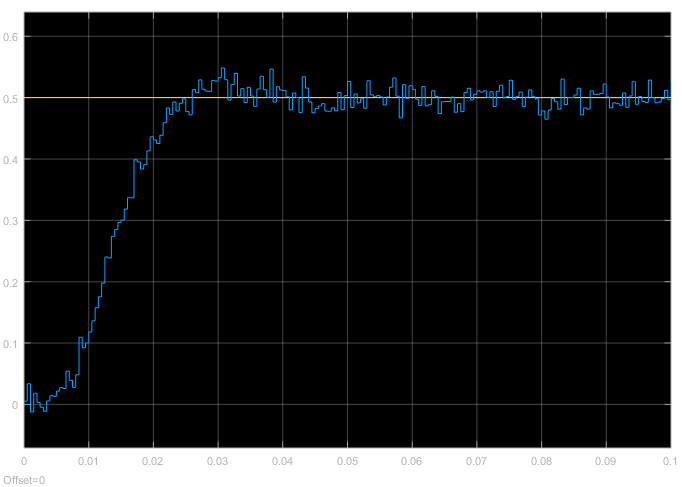
\includegraphics[scale=0.55]{./img/stepCtrlObs_ajustado_2.png}
	\label{fig:stepCtrlObs_ajustado_2}
	\legend{Software: Simulink}
\end{figure}

\begin{figure}[htb!]
	\centering
	\caption{Ação de controle após ajuste de polos não dominantes.}
	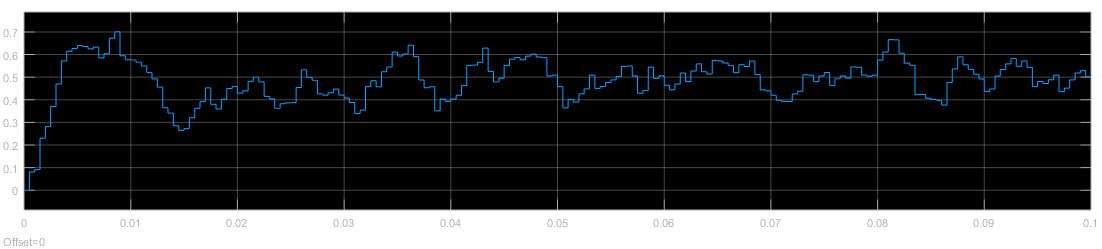
\includegraphics[scale=0.6]{./img/stepCtrlObs_wng_ajustado_ctrlAction.png}
	\label{fig:stepCtrlObs_wng_ajustado_ctrlAction}
	\legend{Software: Simulink}
\end{figure}

\pagebreak

Após ajustes a resposta do sistema apresentou o seguinte sobressinal e tempo de acomodação:
$$
\zeta = 0.60
$$
$$
t_s = 20 ms
$$
$$
j=
\left[
\begin{array}{cccc}
150+j176.5 &  150-j176.5 & -250 & -250
\end{array}
\right]
$$
\begin{figure}[htb!]
	\centering
	\caption{Resposta ao degrau do sistema após ajustes do controlador.}
	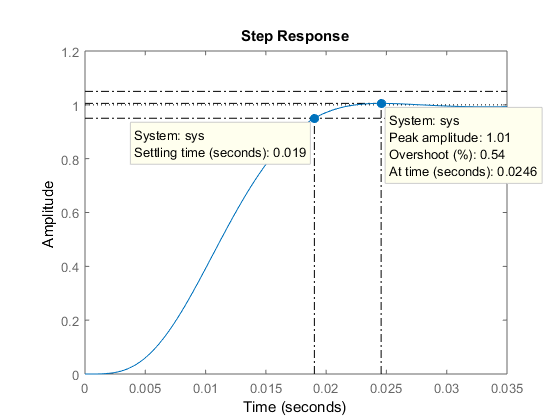
\includegraphics[scale=0.8]{./img/respStepAjusts.png}
	\label{fig:respStepAjusts}
	\legend{Software: MATLAB}
\end{figure}

\pagebreak

\section{\textbf{Implementação recursiva do controlador no Espaço de Estados.}}

\subsection{Análise em simulação da equação recursiva.}

O \autoref{app:implementacaoRecursivaMATLAB} apresenta uma implementação de simulação na forma recursiva do controlador para ser executado no MATLAB. 
Os resultados da simulação: \autoref{fig:resultadoDaEqRecursiva} apresenta a resposta ao degrau e ação de controle e a \autoref{fig:estadosEamostragem} apresenta os estados da planta. Os resultados apresentados são coerentes com as simulações feitas nas seções anteriores.

\begin{figure}[htb!]
	\centering
	\caption{Resposta ao degrau do sistema compensado.}
	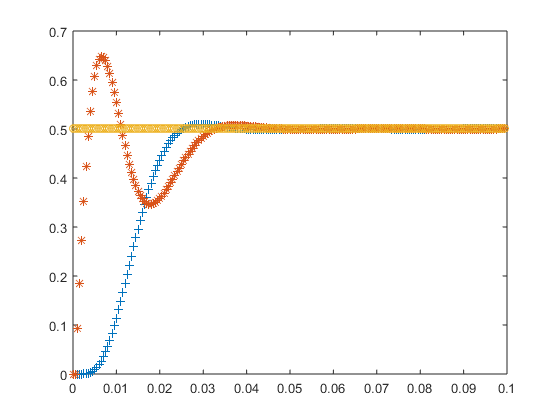
\includegraphics[scale=0.65]{./img/resultadoDaEqRecursiva.png}
	\label{fig:resultadoDaEqRecursiva}
	\legend{Software: Simulink}
\end{figure}

Como o controlador é uma versão discretizada de um projeto de tempo contínuo, a frequência de amostragem de $2 kHz$ foi escolhida de tal forma a manter a resolução do estado mais rápido do sistema. Dessa forma o sistema se manteve estável.

\begin{figure}[htb!]
	\centering
	\caption{Resposta ao degrau do sistema compensado.}
	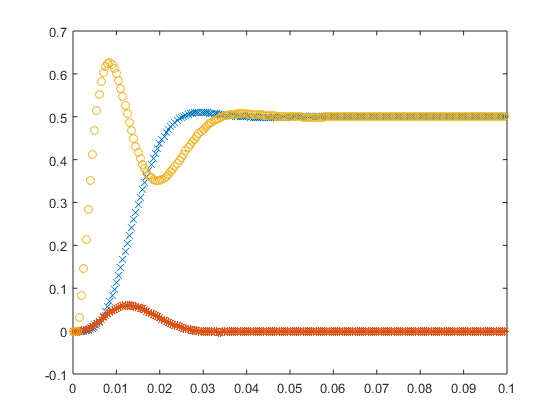
\includegraphics[scale=0.65]{./img/estadosEamostragem.png}
	\label{fig:estadosEamostragem}
	\legend{Software: Simulink}
\end{figure}

\pagebreak

\subsection{Implementação da equação recursiva com a biblioteca CMSIS.}

O pacote CMSIS é um conjunto de bibliotecas desenvolvidas pela Keil otimizadas para os processadores de arquitetura ARM \cite{CMSISDSPReference}.
Essa biblioteca apresenta um conjunto de ferramentas para operações com matriz que facilitam os projetos de controladores no espaço de estados.
O \autoref{app:implementacaoRecursivaCMSIS} apresenta a implementação do controlador na forma recursiva a ser executado pelo microcontrolador e o \autoref{app:firmwareCompleto} apresenta o \textit{firmware} completo.


\pagebreak

\subsection{Análise dos resultados experimentais.}

Como o sobressinal apresentado se mostrou com amplitude igual a $5\%$, foram medidos dois casos: Com tempo de acomodação acontecendo antes do tempo de sobressinal, \autoref{fig:ts5Ampli_before} e \autoref{fig:ts5_before}; e com o tempo de acomodação acontecendo ao mesmo tempo que o sobressinal, \autoref{fig:ts5Ampli_after} e \autoref{fig:ts5_after}.

\begin{figure}[htb!]
	\centering
	\caption{Resposta ao degrau do sistema compensado.}
	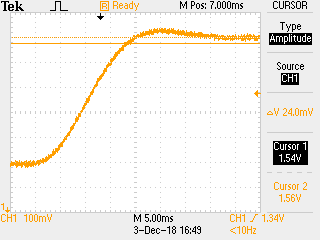
\includegraphics[scale=1.2]{./img/ts5Ampli_before.png}
	\label{fig:ts5Ampli_before}
	\legend{Osciloscópio Tektronics Tds1002c}
\end{figure}

\begin{figure}[htb!]
	\centering
	\caption{Resposta ao degrau do sistema compensado.}
	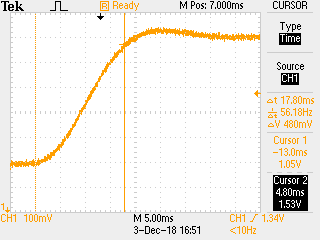
\includegraphics[scale=1.2]{./img/ts5_before.png}
	\label{fig:ts5_before}
	\legend{Osciloscópio Tektronics Tds1002c}
\end{figure}

\pagebreak

\begin{figure}[htb!]
	\centering
	\caption{Resposta ao degrau do sistema compensado.}
	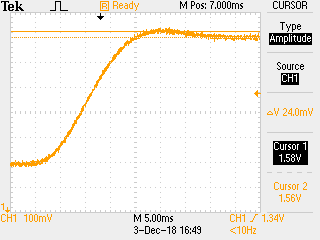
\includegraphics[scale=1.2]{./img/ts5Ampli_after.png}
	\label{fig:ts5Ampli_after}
	\legend{Osciloscópio Tektronics Tds1002c}
\end{figure}

\begin{figure}[htb!]
	\centering
	\caption{Resposta ao degrau do sistema compensado.}
	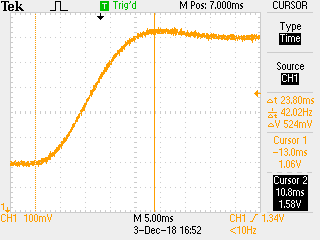
\includegraphics[scale=1.2]{./img/ts5_after.png}
	\label{fig:ts5_after}
	\legend{Osciloscópio Tektronics Tds1002c}
\end{figure}

\pagebreak

A \autoref{tab:tabelaResultados} apresenta um comparativo entre resultados simulados e experimentais.
Para o caso onde a amplitude onde ocorre o sobressinal for considerada como $5\%$, o projeto extrapolou o requisito de tempo em $30 \mu s$. Um pequeno ajuste no sobressinal, para tornar esse um pouco menor que $5\%$, diminuiria o tempo de acomodação de forma a cumprir o requisito de projeto.

\begin{table}[htbp]
\caption{Tabela comparativa de resultados.}
\begin{center}
\begin{tabular}{|l|l|l|l|l|l|}
\hline
 & Simulação & Experimental & Experimental & Requisitos & Planta (FTMA) \\ \hline
$M_p$ (\%) & $0.54$ & se $M_p<5\%$ & $5.0$ & $10.0$ & $20.0$ \\ \hline
$T_{s5\%}$ (ms) & $19.0$ & $17.8$ & $23.8$ & $23.4$ & $46.7$ \\ \hline
\end{tabular}
\end{center}
\label{tab:tabelaResultados}
\end{table}

A \autoref{fig:tempoDeProcessamento} mostra a aquisição do tempo de processamento de cada ciclo de execução do controlador. O tempo de processamento durou aproximadamente $76 \mu s$.
\begin{figure}[htb!]
	\centering
	\caption{Tempo de processamento.}
	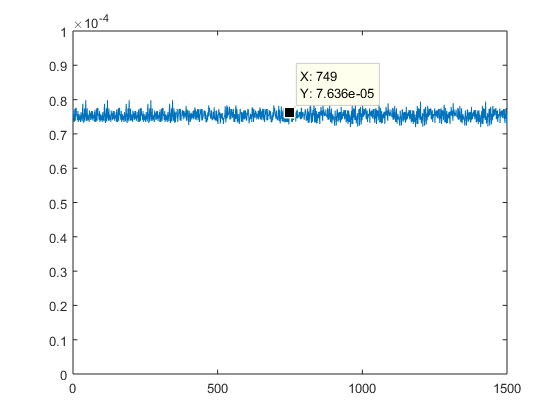
\includegraphics[scale=0.8]{./img/tempoDeProcessamento.png}
	\label{fig:tempoDeProcessamento}
	\legend{Software: MATLAB}
\end{figure}

\pagebreak

\section{\textbf{Conclusão}}
 
Técnicas de projeto de controladores no espaço de estados são uma poderosa ferramento para se trabalhar com sistemas de múltiplas entras e saídas. Porém para sistemas de apenas uma entrada e saída apresentam resultados similares a projetos de controladores discretos com funções transferências no domínio da transformada Z. Se for trabalhada a abordagem da discretização do controlador calculado com variáveis contínuas, há uma necessidade de frequências de amostragens relativamente maiores que os controladores de funções transferências.

Se a planta a ser controlada permitir a leitura de seus estados, a sequência de código a ser processado pelo microcontrolador se torna pequena, porém se surge a necessidade do processamento de um observador de estados, a demanda de processamento aumenta devido ao grande volume de operações com matrizes.

Para aplicações simples controladores baseados em funções transferências parecem se equivaler aos controladores no espaço de estado, porém para aplicações mais complexas o espaço de estado definitivamente será um poderoso caminho.
%
%
%
%
\pagebreak

% ----------------------------------------------------------
% ELEMENTOS PÓS-TEXTUAIS
% ----------------------------------------------------------
\postextual

% ---
% Título e resumo em língua estrangeira
% ---

% ----------------------------------------------------------
% Referências bibliográficas
% ----------------------------------------------------------
\bibliography{bib_eletronic.eng}

% ----------------------------------------------------------
% Glossário
% ----------------------------------------------------------
%
% Há diversas soluções prontas para glossário em LaTeX. 
% Consulte o manual do abnTeX2 para obter sugestões.
%
%\glossary

% ----------------------------------------------------------
% Apêndices
% ----------------------------------------------------------

% ---
% Inicia os apêndices
% ---
\begin{apendicesenv}
	
	% Imprime uma página indicando o início dos apêndices
	\partapendices

\chapter{Controlador recursivo do sistema de controle com observador de ordem plena implementada no MATLAB}
% ----------------------------------------------------------
	\label{app:implementacaoRecursivaMATLAB}
	
	\lstset{language=MATLAB}
	\begin{lstlisting}
%% ========================================================================
% Equacao Recursiva: Planta e Observador:
plotSize = 200;
k = 0:plotSize-1; kT = k*T;

r = zeros(1, plotSize); r(1:plotSize) = 0.5;
y = zeros(1, plotSize);
u = zeros(1, plotSize);

erro_I_dot = zeros(1, plotSize);
erro_I = zeros(1, plotSize);

x_obs = zeros(3, plotSize);
x_dot_obs = zeros(3, plotSize);

x_planta = zeros(3, plotSize);
x_dot_planta = zeros(3, plotSize);

for n=2:plotSize
    %%---------------------------------
    %Integrador para fazer a planta do tipo 0 se tornar do tipo 1:
        erro_I(n) = T*erro_I_dot(n-1)+ erro_I(n-1);
    %%---------------------------------
    %%---------------------------------
    %Observador:
        x_obs(:, n) = T*x_dot_obs(:, n-1) + x_obs(:, n-1);
    %%---------------------------------
    Kx = K*x_obs(:, n);
    
    %Acao de controle:
    u(n) = KI*erro_I(n) - Kx;
    
    %%=================================
    %Planta:
        %%---------------------------------
            x_planta(:, n) = T*x_dot_planta(:, n-1) + x_planta(:, n-1);
        %%---------------------------------
        x_dot_planta(:, n) = B*u(n) + A*x_planta(:, n);
        y(n) = C*x_planta(:, n);%Saida da planta:
    %%=================================
    
    erro_I_dot(n) = r(n) - y(n);
    Bu_obs_1 = B*u(n);
    erro_obs = y(n) - C*x_obs(:, n);
    Key = erro_obs*Ke;
    Bu_obs_2 = Bu_obs_1 + Key;
    x_dot_obs(:, n) = Bu_obs_2 + A*x_obs(:, n);
end

figure(6); plot(kT, y, '+'); hold on
plot(kT, u, '*'); hold on
plot(kT, r, 'o') 
% ylim([-0.1 1])
hold off
	\end{lstlisting}
	\pagebreak

\chapter{Controlador recursivo do sistema de controle com observador de ordem plena implementada no microcontrolador}
% ----------------------------------------------------------
	\label{app:implementacaoRecursivaCMSIS}
	
	\lstset{language=C}
	\begin{lstlisting}
void sampler_ss_state_process()
{
    //*******************************************************************
    //Counter Start:
    Timer_1_WriteCounter(1000000);
    //*******************************************************************
    main_state = STANDBY_STATE;      
    //-------------------------------------------------------------------
    //===================================================================    
    erro_I = SAMPLE_RATE*erro_I_dot + erro_I;
    
    arm_mat_scale_f32(&x_dot_obs, SAMPLE_RATE, &x_dot_obs);
    arm_mat_add_f32(&x_dot_obs, &x_obs, &x_obs);
    arm_mat_mult_f32(&K, &x_obs, &Kx);
       
    u = KI*erro_I - Kx.pData[0];     
    
    //===================================================================  
    outputBuffer = (uint16)(u*0xfff);   
    PWM_WriteCompare(outputBuffer);        
    adcBuffer = ADC_SAR_GetResult16(); 
    y=((float32)adcBuffer)/(0xfff);   
    //===================================================================  
    
    erro_I_dot = inputBuffer - y;
    
    arm_mat_scale_f32(&B_obs, u, &Bu_obs_1);
    
    arm_mat_mult_f32(&C_obs, &x_obs, &y_obs);
    erro_obs = y - y_obs.pData[0];
    
    arm_mat_scale_f32(&Ke, erro_obs, &Key);
    arm_mat_add_f32(&Bu_obs_1, &Key, &Bu_obs_2);
    
    arm_mat_mult_f32(&A_obs, &x_obs, &Ax_obs);
    arm_mat_add_f32(&Bu_obs_2, &Ax_obs, &x_dot_obs);    
    //-------------------------------------------------------------------
//    uartOut_array[0]=outputBuffer;
//    uartOut_array[1]=outputBuffer>>8;
    uartOut_array[0]=adcBuffer;
    uartOut_array[1]=adcBuffer>>8;
    UART_1_PutArray(uartOut_array, 2); 
  
    //*******************************************************************
    //Counter End:
    cycleCounter = Timer_1_ReadCounter(); 
    //******************************************************************* 
    
//    uartOut_array[0]=cycleCounter;
//    uartOut_array[1]=cycleCounter>>8;
//    uartOut_array[2]=cycleCounter>>16;
//    uartOut_array[3]=cycleCounter>>24;
//    UART_1_PutArray(uartOut_array, 4);     
}
	\end{lstlisting}
	\pagebreak

\chapter{Firmware Completo}
% ----------------------------------------------------------
	\label{app:firmwareCompleto}
	
	\lstset{language=C}
	\begin{lstlisting}
#include "project.h" 
#include "arm_math.h"

// -----------------------------------------------------------------------------
#define SAMPLE_RATE 500e-06

#define OFF_COMMAND 0x00
#define FULL_COMMAND  0xff

#define ENABLE_COMMAND 0b00000001 
#define RESET_COMMAND  0b00000010

#define CLOSELOOP_COMMAND 0b00000100
#define COMP_ON_COMMAND   0b00001000
#define ZPSYS_ON_COMMAND  0b00010000
uint32 streamSys_status;

uint8 uartOut_array[6];
uint16 adcBuffer, outputBuffer;
uint32 cycleCounter;
float32 adcBufferFloat, erroBuffer, inputBuffer;

// -----------------------------------------------------------------------------
// Transfer Function Controller Buffers
float32 Gc_inputBuffer[2], Gc_outputBuffer[2], Gc_K = 2.5389, Gc_beta=-0.3892, Gc_alpha=-0.4663;
float32 sys_inputBuffer[3], sys_outputBuffer[3];

// -----------------------------------------------------------------------------
// Space State Controller Buffers
float32 r;
float32 erro_I_dot, erro_I, erro_obs;
float32 u;
float32 y;

float32 x_dot_planta_F32[3];
arm_matrix_instance_f32 x_dot_planta;
float32 x_planta_F32[3];
arm_matrix_instance_f32 x_planta;
float32 Bu_planta_F32[3];
arm_matrix_instance_f32 Bu_planta;
float32 Ax_planta_F32[3];
arm_matrix_instance_f32 Ax_planta;
float32 y_planta_F32[1];
arm_matrix_instance_f32 y_planta;

float32 Key_F32[3];
arm_matrix_instance_f32 Key;
const float32 Ke_F32[3]={460.1461, 329.5582, -457.3230};
arm_matrix_instance_f32 Ke;

float32 x_dot_obs_F32[3];
arm_matrix_instance_f32 x_dot_obs;
float32 x_obs_F32[3];
arm_matrix_instance_f32 x_obs;
float32 Bu_obs_1_F32[3];
arm_matrix_instance_f32 Bu_obs_1;
float32 Bu_obs_2_F32[3];
arm_matrix_instance_f32 Bu_obs_2;
float32 Ax_obs_F32[3];
arm_matrix_instance_f32 Ax_obs;
float32 y_obs_F32[1];
arm_matrix_instance_f32 y_obs;


const float32 A_F32[9]={0, 625, 0, -21.6263, -113.5381, 21.6263, 0, 0, -526.3158};
arm_matrix_instance_f32 A_obs;//{0, 1, 0; 0, 0, 1; -7142000, -6.928571000000000e4, -6.229300000000000e2};
const float32 B_F32[9]={0, 0, 526.3158};
arm_matrix_instance_f32 B_obs;
const float32 C_F32[9]={1, 0, 0};
arm_matrix_instance_f32 C_obs;

const float32 KI = 601.0964;
const float32 K_F32[3]={6.1402, 16.6454, 0.3043};
arm_matrix_instance_f32 K;
float32 Kx_F32[1];
arm_matrix_instance_f32 Kx;

float32 INT1_BufferX_F32[3], INT1_BufferY_F32[3];
arm_matrix_instance_f32 int1_BufferX, int1_BufferY;
void arm_mat_integrator_f32(arm_matrix_instance_f32 *pX, arm_matrix_instance_f32 *pBufferX, arm_matrix_instance_f32 *pY, arm_matrix_instance_f32 *pBufferY);

float32 INT2_BufferX_F32; float32 INT2_BufferY_F32;
void arm_integrator_f32(float32 pX, float32* pBufferX, float32* pY, float32* pBufferY);

void arm_mat_integrator_f32(arm_matrix_instance_f32 *pX, arm_matrix_instance_f32 *pBufferX, arm_matrix_instance_f32 *pY, arm_matrix_instance_f32 *pBufferY)
{
    arm_mat_scale_f32(pBufferX, SAMPLE_RATE, pBufferX);
    arm_mat_add_f32(pBufferX, pBufferY, pY);
    arm_copy_f32(pY->pData, pBufferY->pData, pBufferY->numRows*pBufferY->numCols);
    arm_copy_f32(pX->pData, pBufferX->pData, pBufferY->numRows*pBufferY->numCols);
}

void arm_integrator_f32(float32 pX, float32* pBufferX, float32* pY, float32* pBufferY)
{
    *pY = SAMPLE_RATE*(*pBufferX) + *pBufferY;
    *pBufferY = *pY;
    *pBufferX = pX;
}
// -----------------------------------------------------------------------------
// State Machine ---------------------------------------------------------------
void exit_state_process();
void start_state_process();
void ss_init_state_process();
void standby_state_process();
void scanOn_state_process();
void scanOff_state_process();
void sampler_tf_state_process();
void sampler_ss_state_process();
void simul_ss_state_process();
void simul2_ss_state_process();
void closeLoop_state_process();
void openLoop_state_process();
void compOn_state_process();
void compOff_state_process();
void zpsysOn_state_process();
void zpsysOff_state_process();
void ctrlOn_state_process();
void ctrlOff_state_process();

//Estado comum a todas as máquinas de estado:
enum statesOfmachine{
    EXIT_STATE = 0,
    START_STATE,
    SS_INIT_STATE,
    STANDBY_STATE,
    SCANON_STATE,
    SCANOFF_STATE,
    SAMPLER_TF_STATE,
    SAMPLER_SS_STATE,
    SIMUL_SS_STATE,
    SIMUL2_SS_STATE,
    CLOSELOOP_STATE,
    OPENLOOP_STATE,
    COMPON_STATE,
    COMPOFF_STATE,
    ZPSYSON_STATE,
    ZPSYSOFF_STATE,
    CTRLON_STATE,
    CTRLOFF_STATE
};

void (*main_state_table[])()=
{
    exit_state_process,
    start_state_process,
    ss_init_state_process,
    standby_state_process,
    scanOn_state_process,
    scanOff_state_process,
    sampler_tf_state_process,
    sampler_ss_state_process,
    simul_ss_state_process,
    simul2_ss_state_process,
    closeLoop_state_process,
    openLoop_state_process,
    compOn_state_process,
    compOff_state_process,
    zpsysOn_state_process,
    zpsysOff_state_process,
    ctrlOn_state_process,
    ctrlOff_state_process
};

volatile int main_state;

CY_ISR(samplerInterrupt_handler)
{	
    main_state =  SAMPLER_SS_STATE;
}

CY_ISR(RxInterrupt_1)
{	
    main_state = UART_1_GetChar();
}

CY_ISR(stepInterrupt_handler)
{	
    //inputBuffer = 0.666;
    inputBuffer = 0.345;
    //inputBuffer = 1;
    //inputBuffer = 0.420;
}

CY_ISR(zeroInterrupt_handler)
{	
    //inputBuffer = 0.333;
    inputBuffer = 0.23;
    //inputBuffer = 0;
    //inputBuffer = 0.150;
}

int main(void)
{
    CyGlobalIntEnable; /* Enable global interrupts. */

    UART_1_Start();
    isr_Rx_1_StartEx(RxInterrupt_1);
     
    isr_SamplerStateSig_StartEx(samplerInterrupt_handler);
    isr_SamplerStateSig_Disable();
    
    isr_stepSig_StartEx(stepInterrupt_handler);
    isr_zeroSig_StartEx(zeroInterrupt_handler);
    
    Control_Reg_1_Write(OFF_COMMAND);   
    
    while(1)
    {
        main_state = START_STATE;
        while(main_state)
        {       
            main_state_table[main_state]();
        }
    }
}

void exit_state_process()
{
   isr_SamplerStateSig_Disable();
}

void start_state_process()
{
    main_state = SS_INIT_STATE;
    
    streamSys_status = streamSys_status&(~CLOSELOOP_COMMAND); 
    streamSys_status = streamSys_status&(~COMP_ON_COMMAND);
    streamSys_status = streamSys_status&(~ZPSYS_ON_COMMAND); 
    
    streamSys_status = streamSys_status|CLOSELOOP_COMMAND;
    streamSys_status = streamSys_status|COMP_ON_COMMAND;
    streamSys_status = streamSys_status|ZPSYS_ON_COMMAND;  
    
    Control_Reg_1_Write(OFF_COMMAND);
    
    Timer_1_Start();
}

void ss_init_state_process()
{
    main_state = STANDBY_STATE;
    
    arm_mat_init_f32(&A_obs, 3, 3, (float32_t *)A_F32);
    arm_mat_init_f32(&B_obs, 3, 1, (float32_t *)B_F32);
    arm_mat_init_f32(&C_obs, 1, 3, (float32_t *)C_F32);
    
    arm_mat_init_f32(&K, 1, 3, (float32_t *)K_F32);
    arm_mat_init_f32(&Kx, 1, 1, (float32_t *)Kx_F32);
    arm_mat_init_f32(&Key, 3, 1, (float32_t *)Key_F32);
    arm_mat_init_f32(&Ke, 3, 1, (float32_t *)Ke_F32);
    
    arm_mat_init_f32(&x_dot_planta, 3, 1, (float32_t *)x_dot_planta_F32);
    arm_mat_init_f32(&x_planta, 3, 1, (float32_t *)x_planta_F32);
    arm_mat_init_f32(&Bu_planta, 3, 1, (float32_t *)Bu_planta_F32);
    arm_mat_init_f32(&Ax_planta, 3, 1, (float32_t *)Ax_planta_F32);
    arm_mat_init_f32(&y_planta, 1, 1, (float32_t *)y_planta_F32);

    arm_mat_init_f32(&x_dot_obs, 3, 1, (float32_t *)x_dot_obs_F32);
    arm_mat_init_f32(&x_obs, 3, 1, (float32_t *)x_obs_F32);
    arm_mat_init_f32(&Bu_obs_1, 3, 1, (float32_t *)Bu_obs_1_F32);
    arm_mat_init_f32(&Bu_obs_2, 3, 1, (float32_t *)Bu_obs_2_F32);
    arm_mat_init_f32(&Ax_obs, 3, 1, (float32_t *)Ax_obs_F32);
    arm_mat_init_f32(&y_obs, 1, 1, (float32_t *)y_obs_F32);
    
    arm_mat_init_f32(&int1_BufferX, 3, 1, (float32_t *)INT1_BufferX_F32);
    arm_mat_init_f32(&int1_BufferY, 3, 1, (float32_t *)INT1_BufferY_F32);
}

void standby_state_process()
{
    
}

void scanOn_state_process()
{
    main_state = STANDBY_STATE;
    
    isr_SamplerStateSig_Enable();
    
    isr_stepSig_Enable();
    isr_zeroSig_Enable();
    
    ADC_SAR_Start();
    ADC_SAR_StartConvert();
    PWM_Start();
    PWM_WriteCompare(10);
    
    Control_Reg_1_Write(ENABLE_COMMAND);
}

void scanOff_state_process()
{
    main_state = STANDBY_STATE;
    
    isr_SamplerStateSig_Disable();
    
    ADC_SAR_Stop();
    ADC_SAR_StopConvert();
    
    PWM_Stop();
    
    Control_Reg_1_Write(OFF_COMMAND);   
}

#define CLOSELOOP_COMMAND 0b00000100
#define COMP_ON_COMMAND  0b00001000
#define ZPSYS_ON_COMMAND 0b00010000

void sampler_tf_state_process()
{
    //*******************************************************************
    //Counter Start:
    Timer_1_WriteCounter(1000000);
    //*******************************************************************
    
    main_state = STANDBY_STATE;
   
    //-------------------------------------------------------------------
    adcBuffer = ADC_SAR_GetResult16(); 
    adcBufferFloat=((float32)adcBuffer)/(0xfff);    
    
    //-------------------------------------------------------------------
    //Opened-Loop or Closed-Loop:
    if(streamSys_status&CLOSELOOP_COMMAND)
        erroBuffer = inputBuffer - adcBufferFloat;//Closed-Loop        
    else
        erroBuffer = inputBuffer;
    //-------------------------------------------------------------------

    Gc_inputBuffer[0] = erroBuffer; 
    
    //-------------------------------------------------------------------
    //Compensator ON or OFF:
    if(streamSys_status&COMP_ON_COMMAND)
        Gc_outputBuffer[0] = Gc_K*Gc_inputBuffer[0] + Gc_K*Gc_alpha*Gc_inputBuffer[1] - Gc_beta*Gc_outputBuffer[1];//ON         
    else
        Gc_outputBuffer[0] = Gc_inputBuffer[0];//OFF         
    //-------------------------------------------------------------------    
    sys_inputBuffer[0] = Gc_outputBuffer[0]; 
    //-------------------------------------------------------------------
    if(streamSys_status&ZPSYS_ON_COMMAND)
        sys_outputBuffer[0] =  sys_inputBuffer[0] - 1.478*sys_inputBuffer[1] + 0.6531*sys_inputBuffer[2] + sys_outputBuffer[1];//ON        
    else
        sys_outputBuffer[0] = sys_inputBuffer[0];//OFF                        
    //-------------------------------------------------------------------
  
    outputBuffer = (uint16)(sys_outputBuffer[0]*0xfff);   
    PWM_WriteCompare(outputBuffer);
    

    
    Gc_inputBuffer[1] = Gc_inputBuffer[0];
    Gc_outputBuffer[1] = Gc_outputBuffer[0];
    
    sys_inputBuffer[2] = sys_inputBuffer[1];
    sys_outputBuffer[2] = sys_outputBuffer[1];  
    sys_inputBuffer[1] = sys_inputBuffer[0];
    sys_outputBuffer[1] = sys_outputBuffer[0];     
    //-------------------------------------------------------------------
    

    
//    uartOut_array[0]=outputBuffer;
//    uartOut_array[1]=outputBuffer>>8;

    uartOut_array[0]=adcBuffer;
    uartOut_array[1]=adcBuffer>>8;
    
    //*******************************************************************
    //Counter End:
    cycleCounter = Timer_1_ReadCounter(); 
    //*******************************************************************   
    
//    uartOut_array[2]=cycleCounter;
//    uartOut_array[3]=cycleCounter>>8;
//    uartOut_array[4]=cycleCounter>>16;
//    uartOut_array[5]=cycleCounter>>24;
//    
    UART_1_PutArray(uartOut_array, 2);  
}

void sampler_ss_state_process()
{
    //*******************************************************************
    //Counter Start:
    Timer_1_WriteCounter(1000000);
    //*******************************************************************
    
    main_state = STANDBY_STATE;      
    //-------------------------------------------------------------------
    //===================================================================          
    erro_I = SAMPLE_RATE*erro_I_dot + erro_I;
    
    arm_mat_scale_f32(&x_dot_obs, SAMPLE_RATE, &x_dot_obs);
    arm_mat_add_f32(&x_dot_obs, &x_obs, &x_obs);
    arm_mat_mult_f32(&K, &x_obs, &Kx);
       
    u = KI*erro_I - Kx.pData[0];     
    
//    u = inputBuffer;
    
    //===================================================================  
    outputBuffer = (uint16)(u*0xfff);   
    PWM_WriteCompare(outputBuffer);        
    adcBuffer = ADC_SAR_GetResult16(); 
    y=((float32)adcBuffer)/(0xfff);   
    //===================================================================  
    
    erro_I_dot = inputBuffer - y;
    
    arm_mat_scale_f32(&B_obs, u, &Bu_obs_1);
    
    arm_mat_mult_f32(&C_obs, &x_obs, &y_obs);
    erro_obs = y - y_obs.pData[0];
    
    arm_mat_scale_f32(&Ke, erro_obs, &Key);
    arm_mat_add_f32(&Bu_obs_1, &Key, &Bu_obs_2);
    
    arm_mat_mult_f32(&A_obs, &x_obs, &Ax_obs);
    arm_mat_add_f32(&Bu_obs_2, &Ax_obs, &x_dot_obs);    
    //-------------------------------------------------------------------

 
    
//    uartOut_array[0]=outputBuffer;
//    uartOut_array[1]=outputBuffer>>8;

    uartOut_array[0]=adcBuffer;
    uartOut_array[1]=adcBuffer>>8;
  
    UART_1_PutArray(uartOut_array, 2); 
  
    //*******************************************************************
    //Counter End:
    cycleCounter = Timer_1_ReadCounter(); 
    //******************************************************************* 
    
//    uartOut_array[0]=cycleCounter;
//    uartOut_array[1]=cycleCounter>>8;
//    uartOut_array[2]=cycleCounter>>16;
//    uartOut_array[3]=cycleCounter>>24;
////    
//    UART_1_PutArray(uartOut_array, 4);     
}

void simul_ss_state_process()
{
    //*******************************************************************
    //Counter Start:
    Timer_1_WriteCounter(1000000);
    //*******************************************************************
    
    main_state = STANDBY_STATE;      
    //-------------------------------------------------------------------
    //===================================================================             
    //&x_dot_obs int -> &x_obs
//    arm_mat_integrator_f32(&x_dot_obs, &int1_BufferX, &x_obs, &int1_BufferY);
    arm_mat_scale_f32(&x_dot_planta, SAMPLE_RATE, &x_dot_planta);
    arm_mat_add_f32(&x_dot_planta, &x_planta, &x_planta);
    
    arm_mat_scale_f32(&B_obs, inputBuffer, &Bu_planta);
    
    arm_mat_mult_f32(&A_obs, &x_planta, &Ax_planta);
    
    arm_mat_add_f32(&Bu_planta, &Ax_planta, &x_dot_planta);
    
    arm_mat_mult_f32(&C_obs, &x_planta, &y_planta);
     
    //===================================================================   
    
    adcBuffer=(uint16)(y_planta.pData[0]*0xfff);     
    //-------------------------------------------------------------------

//    uartOut_array[0]=outputBuffer;
//    uartOut_array[1]=outputBuffer>>8;

    uartOut_array[0]=adcBuffer;
    uartOut_array[1]=adcBuffer>>8;
  
    UART_1_PutArray(uartOut_array, 2); 

    //*******************************************************************
    //Counter End:
    cycleCounter = Timer_1_ReadCounter(); 
    //*******************************************************************    
    
    uartOut_array[0]=cycleCounter;
    uartOut_array[1]=cycleCounter>>8;
    uartOut_array[2]=cycleCounter>>16;
    uartOut_array[3]=cycleCounter>>24;
    
    UART_1_PutArray(uartOut_array, 4);     
}

void simul2_ss_state_process()
{
    //*******************************************************************
    //Counter Start:
    Timer_1_WriteCounter(1000000);
    //*******************************************************************
    
    main_state = STANDBY_STATE;      
    //-------------------------------------------------------------------
    //===================================================================          
    erro_I = SAMPLE_RATE*erro_I_dot + erro_I;
    
    arm_mat_scale_f32(&x_dot_obs, SAMPLE_RATE, &x_dot_obs);
    arm_mat_add_f32(&x_dot_obs, &x_obs, &x_obs);
    arm_mat_mult_f32(&K, &x_obs, &Kx);
       
    u = KI*erro_I - Kx.pData[0];   
    outputBuffer=(uint16)(u*0xfff); 
    //===================================================================  
    //&x_dot_obs int -> &x_obs
    arm_mat_scale_f32(&x_dot_planta, SAMPLE_RATE, &x_dot_planta);
    arm_mat_add_f32(&x_dot_planta, &x_planta, &x_planta);
    
    arm_mat_scale_f32(&B_obs, u, &Bu_planta);   
    arm_mat_mult_f32(&A_obs, &x_planta, &Ax_planta);  
    arm_mat_add_f32(&Bu_planta, &Ax_planta, &x_dot_planta);
    
    arm_mat_mult_f32(&C_obs, &x_planta, &y_planta);
    //===================================================================  
    
    erro_I_dot = inputBuffer - y_planta.pData[0];
    
    arm_mat_scale_f32(&B_obs, u, &Bu_obs_1);
    
    arm_mat_mult_f32(&C_obs, &x_obs, &y_obs);
    erro_obs = y_planta.pData[0] - y_obs.pData[0];
    
    arm_mat_scale_f32(&Ke, erro_obs, &Key);
    arm_mat_add_f32(&Bu_obs_1, &Key, &Bu_obs_2);
    
    arm_mat_mult_f32(&A_obs, &x_obs, &Ax_obs);
    arm_mat_add_f32(&Bu_obs_2, &Ax_obs, &x_dot_obs); 
    //===================================================================   
    
    adcBuffer=(uint16)(y_planta.pData[0]*0xfff);     
    //-------------------------------------------------------------------

    uartOut_array[0]=outputBuffer;
    uartOut_array[1]=outputBuffer>>8;

//    uartOut_array[0]=adcBuffer;
//    uartOut_array[1]=adcBuffer>>8;
  
    UART_1_PutArray(uartOut_array, 2); 

    //*******************************************************************
    //Counter End:
    cycleCounter = Timer_1_ReadCounter(); 
    //*******************************************************************    
    
//    uartOut_array[0]=cycleCounter;
//    uartOut_array[1]=cycleCounter>>8;
//    uartOut_array[2]=cycleCounter>>16;
//    uartOut_array[3]=cycleCounter>>24;
////    
//    UART_1_PutArray(uartOut_array, 4);     
}

void closeLoop_state_process()
{
    main_state = STANDBY_STATE;
    streamSys_status = streamSys_status|CLOSELOOP_COMMAND;   
}

void openLoop_state_process()
{
    main_state = STANDBY_STATE;
    streamSys_status = streamSys_status&(~CLOSELOOP_COMMAND);    
}

void compOn_state_process()
{
    main_state = STANDBY_STATE;
    streamSys_status = streamSys_status|COMP_ON_COMMAND; 
}

void compOff_state_process()
{
    main_state = STANDBY_STATE;
    streamSys_status = streamSys_status&(~COMP_ON_COMMAND); 
}

void zpsysOn_state_process()
{
    main_state = STANDBY_STATE;
    streamSys_status = streamSys_status|ZPSYS_ON_COMMAND; 
}

void zpsysOff_state_process()
{
    main_state = STANDBY_STATE;
    streamSys_status = streamSys_status&(~ZPSYS_ON_COMMAND);   
}

void ctrlOn_state_process()
{
    main_state = STANDBY_STATE;
    streamSys_status = streamSys_status|CLOSELOOP_COMMAND;
    streamSys_status = streamSys_status|COMP_ON_COMMAND;
    streamSys_status = streamSys_status|ZPSYS_ON_COMMAND;     
}

void ctrlOff_state_process()
{
    main_state = STANDBY_STATE;
    streamSys_status = streamSys_status&(~CLOSELOOP_COMMAND); 
    streamSys_status = streamSys_status&(~COMP_ON_COMMAND);
    streamSys_status = streamSys_status&(~ZPSYS_ON_COMMAND); 
}
	\end{lstlisting}
	\pagebreak
	
\end{apendicesenv}
% ---

\pagebreak
\end{document}



